%% Quadratic Template Scoring -- IOP Journal LaTeX manuscript
%% REVISION 1 (PMEA-107016) -- all changes relative to the original submission
%% are marked in blue via \rev{...} (see preamble). Deleted/condensed passages
%% are listed in the point-by-point response letter.
\documentclass{iopjournal}

\usepackage{amsmath}
\usepackage{amssymb}
\usepackage{bm}
\usepackage{booktabs}
\usepackage{array}
\usepackage{xcolor}
% --- revision marking: every inserted or changed passage is wrapped in \rev{}
% (\long so that multi-paragraph arguments are allowed; floats stay outside)
\long\def\rev#1{{\color{blue}#1}}
% blue column types for tables whose numeric content changed
\newcolumntype{B}{>{\color{blue}}c}
\newcolumntype{Q}{>{\color{blue}}l}

% --- Override IOP run-in subsubsection so the body returns to roman ---
\makeatletter
\renewcommand\subsubsection{\@startsection{subsubsection}{3}{\z@}%
                                     {-3.25ex\@plus -1ex \@minus -.2ex}%
                                     {1ex\@plus .2ex}%  % positive afterskip: body on new line, normal font
                                     {\reset@font\normalsize\itshape}}
\makeatother

\graphicspath{{figures/}}

\begin{document}

\articletype{Paper}

\title{Quadratic Template Scoring: A Parameter-Efficient Approach to Unsupervised ECG Anomaly Detection}

\author{Jing Shen$^{1}$, Huashun Li$^{2,*}$ and Jian Gao$^{2}$}

\affil{$^1$School of Medicine, Anhui University of Science and Technology, Huainan, China}

\affil{$^2$School of Electrical and Information Engineering, Anhui University of Science and Technology, Huainan, China}

\affil{$^*$Author to whom any correspondence should be addressed.}

\email{413013008@qq.com (J. Shen); 2021200795@aust.edu.cn (H. Li); 1210099343@qq.com (J. Gao)}

\keywords{ECG anomaly detection, unsupervised learning, template matching, quadratic scoring, QT interval}

\begin{abstract}
\textit{Objective.} Unsupervised anomaly detection in 12-lead electrocardiograms (ECGs) enables scalable cardiac screening when only normal recordings are available. Existing deep reconstruction and one-class methods demand large parameter budgets and offer little decision-process insight; we show that a simpler, physiologically aligned baseline matches them.

\textit{Approach.} We propose Quadratic Template Scoring (QTS), a sliding-window vector-quantisation method that learns $M = 64$ templates whose length is aligned with the QT interval (310\,ms) --- the depolarisation--repolarisation window where most diagnostically significant ECG abnormalities manifest. Each recording is scored by the mean over sliding windows of the minimum squared distance to the nearest template; an algebraic expansion realises the entire forward pass as two 1D convolutions, with no activations, attention or decoder. Training minimises the mean best-match score on normal-only data with AdamW. QTS is evaluated on PTB-XL (21\,799 recordings) and CPSC 2018 (6\,877 recordings) under a patient-level 70/15/15 split, against 12 unsupervised baselines over \rev{ten pre-registered seeds (0--9) that are shared by all methods and that determine both initialisation and the patient split}.

\textit{Main results.} \rev{On CPSC 2018, QTS ranks first with an AUROC of $0.840 \pm 0.011$, significantly above all 12 baselines (two-sided paired Wilcoxon signed-rank tests with Holm correction over the ten seeds). On PTB-XL, QTS attains $0.862 \pm 0.008$, second behind Deep SVDD ($0.877 \pm 0.005$; mean difference $-0.015$, 95\% CI $[-0.021, -0.008]$) but significantly above the remaining 11 baselines. QTS uses 119\,K parameters and trains in about 170\,s (PTB-XL) or 17\,s (CPSC 2018) on a single consumer GPU. A scale ablation under the same protocol shows that the QT-interval scale alone matches multi-scale combinations on PTB-XL with one-third of the parameters, while on CPSC 2018 multi-scale variants hold a small ($\approx 0.006$ AUROC) advantage; cross-dataset transfer experiments show that templates trained on CPSC 2018 transfer to PTB-XL without loss (AUROC 0.884). Sub-group analysis shows QTS excels on QRS-altering and ectopic pathologies (MI, PVC, RBBB, IAVB; AUROC 0.79--0.99) and is weaker than Deep SVDD on subtle ST-segment shifts and hypertrophy.}

\textit{Significance.} A physiologically aligned vector-quantisation baseline is competitive with much larger deep models for ECG anomaly screening. Its interpretable, low-cost design suits point-of-care and wearable deployment, and the sub-group analysis clearly indicates the clinical scenarios in which the method can be trusted and those in which it should not. \rev{Code, fixed seed lists and full reproducibility documentation accompany the manuscript and are publicly available at https://github.com/ZS520L/QTS-ECG.}
\end{abstract}

\section{Introduction}

Cardiovascular diseases remain the leading cause of mortality worldwide, responsible for approximately 17.9 million deaths each year (World Health Organization 2023). The 12-lead electrocardiogram (ECG) is the most widely used non-invasive diagnostic tool for cardiac assessment: it is inexpensive, rapid, broadly available across primary, secondary and emergency care, and is routinely acquired during pre-operative assessment, routine physicals and remote/wearable monitoring. The clinical bottleneck is interpretation rather than acquisition. The annual volume of recorded ECGs already exceeds the capacity of trained electrocardiographers in most health systems, and the gap is widening as wearable single-/three-lead devices push acquisition into the consumer space and as low- and middle-income regions struggle with cardiologist shortages. Automated systems that can reliably \emph{triage} recordings --- reserving expert attention for likely-abnormal cases without missing them --- therefore offer direct clinical value, particularly for screening, telemedicine and continuous monitoring scenarios.

This triage task is well suited to \emph{unsupervised} formulation. Pathological labels are expensive, noisy and inevitably incomplete (the prevalence of any individual diagnosis is typically a few percent), whereas normal recordings are abundant and clinically unambiguous. Learning a model of normal cardiac electrophysiology from healthy recordings alone, and flagging deviations at test time, has three clinical advantages over multi-class supervised classification: (i) it generalises to rare and novel pathologies that were not in the training label set; (ii) it produces a continuous anomaly score directly usable for risk stratification and triage thresholding; and (iii) it sidesteps the prohibitive cost of curating a label-balanced dataset across the full long tail of cardiac diagnoses.

\textbf{The ECG is fundamentally a quasi-periodic signal.} A normal recording consists of repeated PQRST complexes --- each heartbeat producing a stereotyped morphological pattern modulated by slow physiological drift. This structure has a crucial implication: \emph{determining whether an ECG is normal reduces to asking whether every local segment matches one of a finite set of normal morphological prototypes.} Indeed, this is precisely how cardiologists reason --- they mentally compare the observed QRS, ST, and T-wave shapes against internalised templates of normality, and flag deviations. \rev{That diagnostically and prognostically relevant information is carried by ECG morphology is also supported by recent clinical ECG-AI studies: deep networks reach cardiologist-level arrhythmia detection from ambulatory ECGs (Hannun et al 2019), screen for ventricular contractile dysfunction from a single sinus-rhythm ECG (Attia et al 2019), automatically diagnose six rhythm and morphology classes across 12 leads (Ribeiro et al 2020), and detect left ventricular hypertrophy with prognostic value in haemodialysis patients (Letz et al 2023). These results motivate morphology-based prototype learning: if morphology carries the diagnostic signal, a model of normal morphology is a natural anomaly detector.} Yet the dominant paradigm in unsupervised ECG anomaly detection --- reconstruction-based or representation-based deep learning --- does not exploit this structure directly.

\rev{\textbf{Why not reconstruction or abstract features?} Autoencoders and their variants score anomalies by reconstruction error, an objective that optimises signal fidelity rather than normality: a sufficiently expressive decoder can reconstruct unseen anomalies almost as well as normal beats (formalised as a worst-case intuition in Section~\ref{sec:theory}). Representation-based methods such as Deep SVDD (Ruff et al 2018) avoid reconstruction but place the decision boundary in an abstract feature space, so a flagged recording cannot be traced back to the morphological feature that caused the flag --- a practical obstacle in clinical deployment, where understanding the reason for a flag is as important as the flag itself.}

These observations motivate a return to the template-matching paradigm --- but in a modern, learnable form. Classical template matching in ECG analysis \rev{(reviewed by Kohler et al 2002)} requires hand-crafted templates, explicit beat segmentation, and fixed similarity thresholds. We ask: \emph{can we retain the simplicity and interpretability of template matching while achieving end-to-end learning and competitive detection performance?}

We instantiate this idea with the \textbf{squared-distance scoring rule} $(\mathbf{x} + \mathbf{w})^2$, which is mathematically equivalent to $\|\mathbf{x} - (-\mathbf{w})\|^2$ and so realises classical vector-quantisation scoring against a learnable codebook (we make this connection precise in Section~\ref{sec:sparse-coding}). Three properties make this rule a convenient choice for learnable template scoring:
\begin{enumerate}
\item \textbf{Exact match criterion.} $(\mathbf{x} + \mathbf{w})^2 = 0$ if and only if $\mathbf{x} = -\mathbf{w}$ at every position. A bank of templates $\{\mathbf{w}_k\}$ thus defines a set of normal prototypes $\{-\mathbf{w}_k\}$, and the minimum over the bank measures how close the input is to any prototype.
\item \textbf{Non-negativity.} The score is always $\geq 0$, giving a natural lower bound on normal data and a monotonically interpretable scale.
\item \textbf{Algebraic decomposability.} Expanding $(\mathbf{x} + \mathbf{w})^2 = \mathbf{x}^2 + 2\mathbf{x}\mathbf{w} + \mathbf{w}^2$ separates the computation into a signal-energy term, a cross-correlation, and a constant --- each implementable as a standard \texttt{conv1d} call. The forward pass thus needs no activation functions, normalisation layers, or decoder.
\end{enumerate}

In this paper, we propose \textbf{Quadratic Template Scoring (QTS)}, which instantiates this idea with a template length explicitly aligned with the QT interval --- the 310\,ms window (155 samples at 500\,Hz) that encompasses a complete depolarisation--repolarisation cycle at typical heart rates. This design is grounded in a key clinical observation: virtually all diagnostically significant ECG abnormalities --- ST elevation/depression, T-wave inversion, QRS widening, QT prolongation --- manifest within the QT interval. Templates are learned end-to-end by minimising the mean best-match score on normal training data, causing them to self-organise into a compact codebook of healthy cardiac morphologies. At inference, anomalous recordings that fail to match any template receive elevated scores.

QTS is evaluated on PTB-XL (Wagner et al 2020) and CPSC 2018 (Liu F et al 2018), two large-scale 12-lead ECG benchmarks with clinically validated labels. The contributions of this work are threefold:
\begin{enumerate}
\item \rev{\textbf{A physiologically aligned vector-quantisation baseline for ECG anomaly detection.} Template matching, dictionary learning and vector quantisation are long-established tools (Linde et al 1980, Aharon et al 2006, Mairal et al 2010), including in their modern learned form (van den Oord et al 2017); our contribution is not the introduction of learnable templates per se, but a systematic instantiation and evaluation of sliding-window vector quantisation at a template length aligned with the QT interval, trained end-to-end on raw 12-lead ECG without beat segmentation and implemented as two standard 1D convolutions. Under a pre-registered ten-seed protocol, this baseline matches or approaches modern deep one-class methods on standard benchmarks. A scale ablation across QRS-only (70\,ms), QT-interval (310\,ms) and full-cycle (630\,ms) templates characterises when a \emph{single} QT-interval scale matches multi-scale variants (PTB-XL) and when it does not (CPSC 2018), identifying the depolarisation--repolarisation window as the dominant --- but not universally sufficient --- diagnostic scale for unsupervised detection.}
\item \rev{\textbf{Competitive empirical performance at order-of-magnitude lower cost, reported honestly.} Over ten pre-registered seeds, QTS attains AUROC $0.862 \pm 0.008$ on PTB-XL and $0.840 \pm 0.011$ on CPSC 2018. On CPSC 2018 it ranks first, significantly above all 12 baselines; on PTB-XL it ranks second, significantly below Deep SVDD ($0.877 \pm 0.005$) by 0.015 AUROC but significantly above the remaining 11 baselines. QTS uses 119\,K parameters --- among the smallest of the deep methods compared --- and trains in about 170\,s (PTB-XL) or 17\,s (CPSC 2018) on a single consumer GPU.}
\item \textbf{Direct interpretability and a transparent map of strengths and limitations.} Each learned template is a 310\,ms ECG waveform that can be inspected, clustered, and overlaid on the input signal, yielding both per-template (``which prototype matched?'') and per-window (``where did the match fail?'') explanations. A sub-group analysis across morphological (MI, RBBB, LBBB, HYP, STTC) and rhythm (CD, AF, PAC, PVC, IAVB) categories shows where the QT-aligned inductive bias helps and where it does not --- \rev{Deep SVDD remains stronger on subtle ST-segment shifts and hypertrophy, and VAE remains competitive on pure-rhythm anomalies} --- providing an honest characterisation of the regime in which QTS is preferable. \rev{A cross-dataset transfer experiment further shows that the learned template bank generalises across cohorts.}
\end{enumerate}

The aim is therefore not to introduce new mathematics but to argue that, once carefully evaluated under a fair patient-level protocol, a physiologically aligned vector-quantisation baseline is competitive with substantially larger deep models and removes much of their apparent advantage on this task.

\section{Related Work}

\subsection{Reconstruction-Based Methods}

Autoencoders (AE) and their variants are the most common approach to unsupervised ECG anomaly detection. A convolutional or recurrent encoder maps the input to a low-dimensional latent vector, and a decoder reconstructs the original signal; the reconstruction error serves as the anomaly score. Variational autoencoders (VAE) (Kingma and Welling 2014) add a probabilistic latent space, while LSTM autoencoders (Malhotra et al 2016) model temporal dependencies explicitly. The spectral-temporal autoencoder (STAE) (Strodthoff et al 2021) operates on both time and frequency representations simultaneously. \rev{Recent ECG-specific work continues this line: a multi-scale masked autoencoder (MMAE-ECG; Zhou Y et al 2025) reports 0.860 detection AUROC on the PTB-XL anomaly-detection benchmark without R-peak pre-processing, and an attention-augmented VAE-BiLSTM (Garreta Basora et al 2025) reports 0.80 AUROC / 0.81 AUPRC on CPSC 2018; we compare against these published numbers in Section~\ref{sec:ecg-specific}.}

\rev{The known weakness of this family --- over-generalisation of the decoder to anomalous inputs --- is analysed as a worst-case geometric intuition in Section~\ref{sec:theory} and empirically in Section~\ref{sec:results}.}

\subsection{Representation-Based Methods}

Deep SVDD (Ruff et al 2018) learns a neural network that maps normal data into a tight hypersphere in feature space; test samples far from the centre are flagged as anomalous. While elegant in principle, the method is sensitive to the choice of network architecture and can suffer from hypersphere collapse. Contrastive learning approaches (Chen et al 2020) learn representations by maximising agreement between augmented views of normal signals, but require careful augmentation design for ECG data. \rev{Notably, an independent neural-architecture search over six unsupervised families on PTB-XL under a 512\,K-parameter budget found Deep SVDD to offer the best Pareto efficiency between detection performance and model size (Ibrahim et al 2025), confirming that Deep SVDD is a particularly strong lightweight baseline on this dataset --- a finding consistent with our own rankings (Section~\ref{sec:results}).}

\subsection{Multi-Scale Convolutional Methods}

Recent work has explored multi-scale 1D convolutions for ECG anomaly detection, using parallel convolutional branches with kernel sizes matched to physiological time scales (QRS complexes, ST-T segments, full cardiac cycles) combined with techniques such as spectral normalisation, channel attention, and feature fusion (Kiranyaz et al 2016, Acharya et al 2017). These architectures achieve strong performance but rely on deep, multi-layer pipelines with many design choices --- activation functions, normalisation strategies, attention mechanisms, data augmentation --- making it difficult to isolate which components are essential.

\subsection{Template Matching in ECG Analysis}

Classical template matching has a long history in ECG processing, primarily for beat classification \rev{and morphology clustering (Kohler et al 2002); by contrast, widely used QRS detectors such as the Pan--Tompkins algorithm operate by band-pass filtering and adaptive thresholding rather than by template comparison (Pan and Tompkins 1985)}. \rev{Correlation-based} methods compare incoming beats against a library of reference morphologies. However, classical approaches require hand-crafted templates, fixed thresholds, and explicit beat segmentation. QTS modernises this paradigm by (i) learning templates end-to-end via gradient descent, (ii) operating on raw multi-lead signals without beat segmentation, (iii) using a principled quadratic scoring function with an efficient convolutional implementation, and (iv) aligning template length with the QT interval to capture the complete depolarisation--repolarisation cycle without requiring explicit beat segmentation.

\subsection{Sparse Coding and Dictionary Learning}\label{sec:sparse-coding}

QTS is best understood as \rev{a physiologically grounded member of} a venerable family of methods --- \textbf{vector quantisation, sparse coding, and dictionary learning} (Linde et al 1980, \rev{Aharon et al 2006,} Mairal et al 2010\rev{, and, in its modern learned form, van den Oord et al 2017}) --- whose theoretical machinery (covering numbers, rate-distortion bounds, online convergence guarantees) has so far seen little use in ECG anomaly detection. Concretely, QTS realises a \emph{one-active-atom} specialisation of dictionary learning: at each sliding-window position, exactly one atom (the best-matching template) is selected, the squared residual is computed, and per-window scores are averaged into a single anomaly score. The \rev{design choices that distinguish QTS from this skeleton are} --- atoms deliberately sized to one \textbf{QT interval} (310\,ms) rather than arbitrary patches, training driven by minimising the \emph{best-match} score on a normal-only set, and an algebraic decomposition that reduces inference to two 1D convolutions.

This combination simultaneously modernises classical ECG template matching \rev{(Kohler et al 2002)} --- replacing hand-crafted dictionaries with learnable ones, fixed thresholds with a continuous score, and explicit beat segmentation with sliding-window aggregation --- while retaining the transparent, prototype-based decision logic that makes template matching clinically interpretable. The methodological message of QTS is therefore not that a new mathematical object has been introduced, but that \textbf{a physiologically aligned dictionary, trained end-to-end with the right scoring rule, recovers a level of performance and transparency that the field had assumed required substantially heavier machinery} --- \rev{matching or approaching the strongest deep one-class baseline on both 12-lead benchmarks (Section~\ref{sec:results}) while using a fraction of the parameter count}.

\rev{\subsection{Recent ECG-Specific Anomaly Detection and Benchmarks}\label{sec:ecg-specific}

Unsupervised and self-supervised anomaly detection tailored to ECG has expanded rapidly. On PTB-XL, MMAE-ECG (Zhou Y et al 2025) combines multi-scale masking with a lightweight transformer encoder and reports 0.860 detection AUROC and 0.749 localisation AUROC at 0.398\,M parameters, removing the heartbeat-segmentation pre-processing of earlier detectors. On CPSC 2018, Garreta Basora et al (2025) benchmark convolutional and recurrent variational autoencoders under a unified pipeline (0.77--0.80 AUROC, 0.80--0.81 AUPRC) and summarise earlier CPSC-2018 comparisons in which a plain VAE reached 0.83 AUROC and a plain AE 0.76. On the method-family level, Ibrahim et al (2025) searched six unsupervised families (Deep SVDD, AE/VAE, masked modelling, normalising flows, diffusion) on PTB-XL under microcontroller constraints and identified Deep SVDD as the Pareto-optimal filter. These studies differ from our protocol in split construction, scoring unit (beat- vs.\ recording-level) and, in part, label usage, so their numbers are not directly comparable to Table~\ref{tab:main}; they do, however, bracket our results (QTS: 0.862 on PTB-XL, 0.840 on CPSC 2018) and independently corroborate two of our empirical findings: the strength of Deep SVDD on PTB-XL and the competitiveness of lightweight, reconstruction-free scoring on ECG.}

\section{Method}

\subsection{Problem Formulation}

Let $\mathbf{x} \in \mathbb{R}^{C \times L}$ denote a 12-lead ECG recording with $C = 12$ channels and $L$ time steps. We are given a training set $\mathcal{D}_\mathrm{train} = \{\mathbf{x}_1, \dots, \mathbf{x}_N\}$ consisting exclusively of normal (healthy) recordings. The goal is to learn a scoring function $S: \mathbb{R}^{C \times L} \to \mathbb{R}_{\geq 0}$ such that $S(\mathbf{x})$ is low for normal recordings and high for anomalous ones.

\subsection{Theoretical Foundation}\label{sec:theory}

\rev{This section formalises the geometric picture underlying QTS. We state up front how these results should be read: the finite-prototype-coverage and intrinsic-dimensionality assumptions below are physiologically plausible but are \emph{not} empirically verified in this work, and the comparison with reconstruction methods is a worst-case statement about unbounded decoder capacity. Propositions 1--4 are therefore intended as formalised intuition and theoretical motivation --- they make the inductive bias of QTS explicit and falsifiable --- rather than as substantive guarantees about trained models on finite data. The empirical case for QTS rests on Sections~\ref{sec:results}--\ref{sec:ablation}.}

\subsubsection{Finite Prototype Coverage Assumption.}

Let $\mathcal{M} \subset \mathbb{R}^{CK}$ denote the manifold of all $K$-sample windows extracted from normal ECG recordings. We assume $\mathcal{M}$ is a compact set with intrinsic dimension $d \ll CK$. This is well-justified by cardiac electrophysiology: normal depolarisation and repolarisation follow constrained ion-channel dynamics, so PQRST morphologies vary smoothly along a few physiological axes (heart rate, electrical axis, amplitude scaling), yielding $d$ on the order of 5--10 even though the ambient dimension $CK = 12 \times 155 = 1{,}860$.

We term the core assumption \emph{finite prototype coverage}: there exists a codebook $\{\boldsymbol{\mu}_k\}_{k=1}^M \subset \mathbb{R}^{CK}$ and a tolerance $\epsilon > 0$ such that for every normal window $\mathbf{x}_t \in \mathcal{M}$,
\begin{equation}
\min_{k} \| \mathbf{x}_t - \boldsymbol{\mu}_k \|^2 \leq \epsilon
\end{equation}
while for windows from anomalous recordings, the minimum distance exceeds $\epsilon$ at a significant fraction of time positions.

\subsubsection{Covering Number Bound on Normal Approximation Error.}

\textbf{Proposition 1} (Prototype sufficiency\rev{; intuition}). \emph{Let $\mathcal{M}$ be a compact $d$-dimensional Riemannian submanifold of $\mathbb{R}^{CK}$ with volume $V$ and reach $\tau > 0$. For any $\epsilon > 0$, the $\epsilon$-covering number of $\mathcal{M}$ satisfies}
\begin{equation}
\mathcal{N}(\mathcal{M}, \epsilon) \leq \frac{V}{\omega_d} \left( \frac{2}{\epsilon} \right)^d
\end{equation}
\emph{where $\omega_d$ is the volume of the unit $d$-ball. Therefore, for $M \geq \mathcal{N}(\mathcal{M}, \epsilon)$ optimally placed prototypes, every normal window is within squared distance $\epsilon^2$ of its nearest prototype.}

\emph{Equivalently, with $M$ prototypes the worst-case approximation error for normal data scales as}
\begin{equation}
\sup_{\mathbf{x} \in \mathcal{M}} \min_{k} \|\mathbf{x} - \boldsymbol{\mu}_k\|^2 = O\!\left( M^{-2/d} \right)
\end{equation}

\emph{Proof sketch.} This follows directly from standard covering number estimates for compact Riemannian manifolds (Niyogi et al 2008). An optimal $\epsilon$-net places prototypes so that the $\epsilon$-balls centred at prototypes cover $\mathcal{M}$. The number of such balls needed is bounded by $V / \mathrm{vol}(B_\epsilon^d)$. The squared-distance bound follows by squaring the covering radius. $\square$

Note that the exponent $-2/d$ depends on the \emph{intrinsic} dimension $d$ rather than the ambient dimension $CK$. Under the (untested) working assumption that $d$ is small for normal ECG windows, even modest values of $M$ may yield a useful covering radius. \rev{(Remark: we do not estimate $d$ empirically; treating it as small is a modelling assumption, and Proposition 1 should be read as a scaling intuition conditional on that assumption.)}

\subsubsection{\rev{Detection Separation Intuition.}}

\textbf{Proposition 2} (Separation gap\rev{; intuition}). \emph{Let $\boldsymbol{\mu}_1, \ldots, \boldsymbol{\mu}_M$ be an $\epsilon$-cover of $\mathcal{M}$. Suppose an anomalous window $\mathbf{x}_a$ satisfies $\mathrm{dist}(\mathbf{x}_a, \mathcal{M}) \geq \delta$ (Euclidean distance to the normal manifold). Then}
\begin{equation}
\min_{k} \|\mathbf{x}_a - \boldsymbol{\mu}_k\|^2 \geq (\delta - \epsilon)^2
\end{equation}
\emph{Consequently, the separation gap between anomalous and normal scores is at least}
\begin{equation}
\Delta \;=\; \min_k \|\mathbf{x}_a - \boldsymbol{\mu}_k\|^2 \;-\; \sup_{\mathbf{x}_n \in \mathcal{M}} \min_k \|\mathbf{x}_n - \boldsymbol{\mu}_k\|^2 \;\geq\; (\delta - \epsilon)^2 - \epsilon^2 \;=\; \delta^2 - 2\delta\epsilon
\end{equation}
\emph{which is strictly positive whenever $\delta > 2\epsilon$.}

\emph{Proof.} By the triangle inequality, for any prototype $\boldsymbol{\mu}_k \in \mathcal{M}_\epsilon$ (the $\epsilon$-neighbourhood of $\mathcal{M}$) and any anomalous window $\mathbf{x}_a$ at distance $\delta$ from $\mathcal{M}$:
\begin{equation}
\|\mathbf{x}_a - \boldsymbol{\mu}_k\| \geq \mathrm{dist}(\mathbf{x}_a, \mathcal{M}) - \mathrm{dist}(\boldsymbol{\mu}_k, \mathcal{M}) \geq \delta - \epsilon
\end{equation}
Squaring and subtracting the normal-data upper bound $\epsilon^2$ gives the result. $\square$
\textbf{Interpretation.} This bound is \emph{architecture-independent}: the separation gap depends only on the manifold geometry ($\delta$, $\epsilon$), not on specific network design choices. In contrast, reconstruction-based methods offer no analogous guarantee --- as we formalise next.

\subsubsection{Reconstruction Methods Lack a Separation Guarantee\rev{ (Worst-Case Intuition)}.}

\textbf{Proposition 3} (Reconstruction failure mode\rev{; worst-case intuition}). \emph{For any compact normal manifold $\mathcal{M}$ and any anomalous point $\mathbf{x}_a \notin \mathcal{M}$, there exists an autoencoder $(f_\theta, g_\theta)$ with a sufficiently expressive decoder $g_\theta$ such that}
\begin{equation}
\|g_\theta(f_\theta(\mathbf{x}_a)) - \mathbf{x}_a\|^2 = 0
\end{equation}
\emph{i.e., the reconstruction error for the anomaly is zero, yielding zero separation.}

\emph{Proof sketch.} Let the encoder $f_\theta$ map $\mathbf{x}_a$ to any latent code $\mathbf{z}_a$, and let the decoder $g_\theta$ be a universal approximator (e.g., a sufficiently wide MLP). Then $g_\theta$ can be constructed to satisfy $g_\theta(\mathbf{z}_a) = \mathbf{x}_a$ while simultaneously minimising reconstruction loss on the training set. This is achievable whenever the latent space has sufficient capacity to encode $\mathbf{x}_a$ without interfering with the encoding of $\mathcal{M}$ --- a mild condition when the bottleneck dimension exceeds $d$. $\square$

\subsubsection{Monotonicity of Detection Performance.}

\textbf{Proposition 4} (Capacity monotonicity\rev{; population-limit intuition}). \emph{Let $S_M(\mathbf{x})$ denote the QTS score with $M$ prototypes trained on normal data.}

\emph{(i) For normal data:} $\sup_{\mathbf{x} \in \mathcal{M}} S_M(\mathbf{x})$ \emph{is non-increasing in $M$ (more prototypes $\Rightarrow$ tighter coverage).}

\emph{(ii) For anomalous data:} $S_M(\mathbf{x}_a) \geq (\delta - \epsilon_M)^2$ \emph{where $\epsilon_M = O(M^{-1/d})$ decreases with $M$, so the anomalous score remains lower-bounded and can only increase as coverage tightens.}

\emph{Consequently, the separation gap $\Delta_M$ is non-decreasing in $M$: detection performance improves monotonically with model capacity.}

\emph{For reconstruction-based methods, this monotonicity does not hold. Increasing decoder capacity can reduce reconstruction error for both normal and anomalous inputs, potentially decreasing $\Delta$.}

\textbf{Summary.} These results sketch a geometric picture in which QTS admits (i) a covering bound that depends on the intrinsic dimension $d$ rather than the ambient dimension $CK$ (Proposition~1, a direct consequence of Niyogi et al 2008), (ii) a separation lower bound $\Delta \geq \delta^2 - 2\delta\epsilon$ between anomalous and normal scores when the cover is tight (Proposition~2), and (iii) monotone non-decrease of this gap as the codebook grows in the population limit (Proposition~4). The corresponding result for reconstruction-based methods (Proposition~3) is a \emph{worst-case} statement under unbounded decoder capacity; in practice, regularisers such as the KL term in VAEs partially mitigate it, as our empirical results in Section~\ref{sec:results} show. We therefore present these propositions as a geometric \emph{intuition} rather than a tight characterisation, \rev{and we label them as such in their statements; their assumptions (compactness, intrinsic dimension, $\epsilon$-coverage of a learned codebook) are working hypotheses that future work could test directly, e.g.\ by estimating the intrinsic dimension of normal ECG window manifolds,} and rely on the experiments below to argue that the inductive bias materialises in practice.

To situate QTS within the broader landscape of unsupervised anomaly detection paradigms, Figure~\ref{fig:paradigm} contrasts QTS with seven other major paradigms covered by our baseline suite: Deep SVDD (one-class boundary in feature space), Autoencoder (reconstruction), TranAD (forecasting), DAGMM (density estimation), BeatGAN (adversarial reconstruction), OC-SVM (kernel boundary), and Isolation Forest (tree-based partitioning). Each paradigm is illustrated with its core mechanism, scoring function, and characteristic failure mode. \rev{We stress that the failure modes shown are \emph{characteristic}, not universal: every paradigm in Figure~\ref{fig:paradigm} has demonstrated strengths in its original application domain (e.g., forecasting-based scoring for smooth sensor drift, density estimation for low-dimensional telemetry, tree ensembles for tabular screening), and several remain competitive in our own experiments --- VAE ranks third on PTB-XL and Isolation Forest is extremely cheap to fit. QTS likewise has limitations, quantified in Sections~\ref{sec:subgroup}--\ref{sec:limitations}; the figure should be read as a map of inductive biases and their characteristic risks, not as a ranking.}

\begin{figure}
\centering
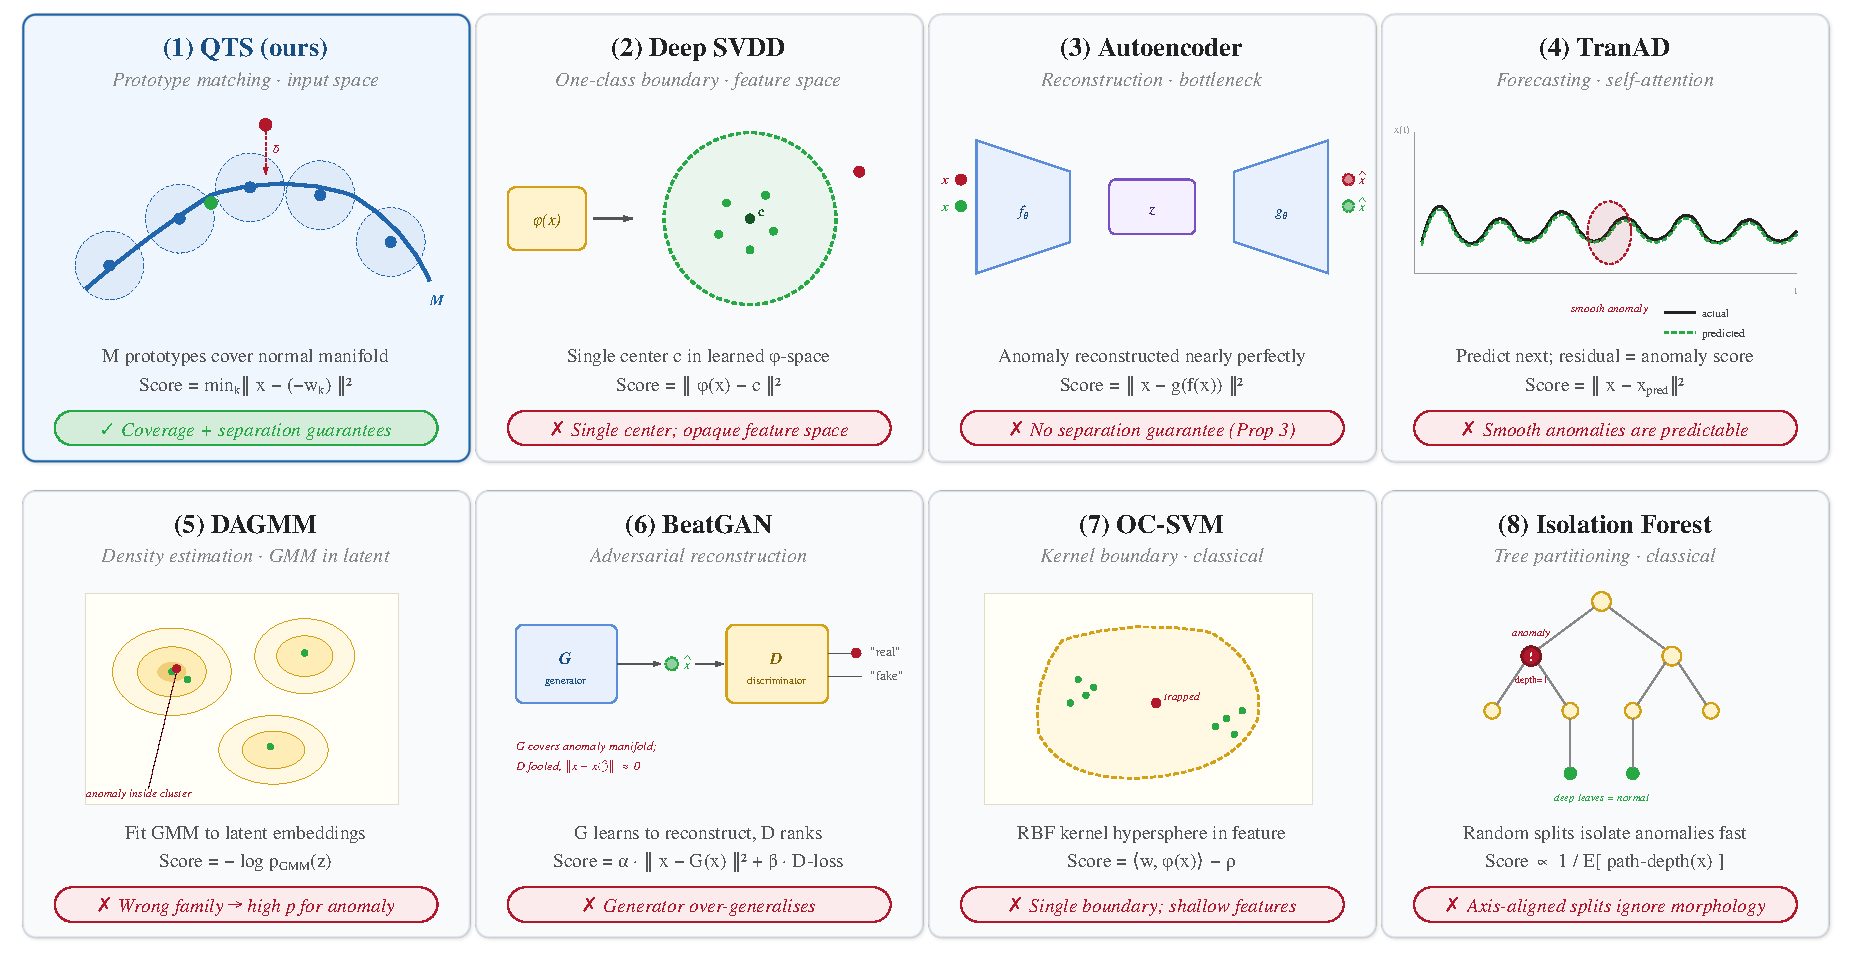
\includegraphics[width=\textwidth]{fig_paradigm_taxonomy.pdf}
\caption{\rev{Eight paradigms of unsupervised anomaly detection on ECG, each with its core mechanism, a characteristic strength, and a characteristic failure mode. (1) QTS (ours): $M$ prototypes cover the normal manifold directly in input space --- strength: inspectable ECG-waveform codebook and per-window explanations; risk: subtle, distributed deviations below the sample-wise noise floor. (2) Deep SVDD: a single hypersphere centre $c$ in a learned feature space --- strength: strong, compact one-class boundary (best PTB-XL AUROC here); risk: mode collapse and no input-space interpretability. (3) Autoencoder: reconstruction objective --- strength: simple, general-purpose; risk: no separation guarantee (Proposition~3). (4) TranAD: forecasting-based residual scoring --- strength: sensitive to local prediction breaks; risk: fooled by smooth anomalies. (5) DAGMM: GMM density in latent space --- strength: probabilistic scores; risk: wrong distributional family yields high likelihood for anomalies. (6) BeatGAN: adversarial generator --- strength: robust to augmentation-rich regimes; risk: over-generalisation covers anomalous morphologies. (7) OC-SVM: kernel boundary --- strength: convex, parameter-light; risk: cannot capture multimodal normal distributions. (8) Isolation Forest: tree-based partitioning --- strength: near-zero training cost; risk: axis-aligned splits ignore morphological structure.}}
\label{fig:paradigm}
\end{figure}

Among these paradigms, QTS is unusual in computing the anomaly score directly in the \textbf{input space} against a \textbf{bank of multiple learnable prototypes}, rather than in a learned feature, latent, reconstruction or partition space. The remaining sections argue that this design choice, when combined with QT-interval alignment, performs comparably to or better than the strongest deep baseline on our benchmarks, while offering more direct interpretability.

\subsection{Quadratic Template Scoring}

\subsubsection{Single-Scale Formulation.}

We maintain a bank of $M$ learnable templates $\{\mathbf{w}_k\}_{k=1}^M$, where each $\mathbf{w}_k \in \mathbb{R}^{C \times K}$ has the same channel dimension as the input and a temporal extent of $K$ samples.

For a sliding window starting at position $t$, we define the per-template score as the sum of squared element-wise deviations:
\begin{equation}
s_{k,t} = \sum_{c=1}^{C} \sum_{i=0}^{K-1} \left( x_{c, t+i} + w_{k, c, i} \right)^2
\end{equation}
This quadratic form achieves its minimum value of zero if and only if $x_{c, t+i} = -w_{k, c, i}$ for all channels and positions simultaneously. In other words, the template $\mathbf{w}_k$ represents the negation of the signal pattern it is designed to match.

The sequence-level score aggregates over templates and time:
\begin{equation}
S(\mathbf{x}) = \frac{1}{T} \sum_{t=0}^{T-1} \min_{k \in \{1, \dots, M\}} \; s_{k, t}
\end{equation}
where $T = \lfloor (L - K) / \mathrm{stride} \rfloor + 1$ is the number of windows. The $\min$ operator selects the best-matching template at each position, and the mean aggregates across the signal.

\subsubsection{Efficient Convolutional Implementation.}

A na\"ive implementation would explicitly unfold every $K$-length window and compute the squared distance to each template, requiring $O(B \cdot M \cdot C \cdot K \cdot T)$ memory for the intermediate tensor. We show that the quadratic form admits an exact algebraic decomposition into standard convolutional operations, avoiding this materialisation entirely.

Starting from the per-template, per-window score:
\begin{equation}
s_{k,t} = \sum_{c=1}^{C} \sum_{i=0}^{K-1} (x_{c,t+i} + w_{k,c,i})^2
\end{equation}
Expanding the square yields three terms:
\begin{equation}
s_{k,t} = \underbrace{\sum_{c,i} x_{c,t+i}^2}_{E_t} + \; 2 \underbrace{\sum_{c,i} x_{c,t+i} \cdot w_{k,c,i}}_{\langle \mathbf{w}_k, \mathbf{x}_t \rangle} + \underbrace{\sum_{c,i} w_{k,c,i}^2}_{\|\mathbf{w}_k\|^2}
\end{equation}
Each term maps to a well-known operation:

\textbf{Term 1 --- Window energy} $E_t = \sum_{c,i} x_{c,t+i}^2$. This is independent of the template index $k$ and depends only on the input. It can be computed as a 1D convolution of $\mathbf{x}^2$ (element-wise square) with an all-ones kernel $\mathbf{1} \in \mathbb{R}^{1 \times C \times K}$:
\begin{equation}
E_t = \mathrm{conv1d}(\mathbf{x} \odot \mathbf{x}, \; \mathbf{1}, \; \mathrm{stride}=s) \qquad \text{shape: } (B, 1, T)
\end{equation}

\textbf{Term 2 --- Cross-correlation} $\langle \mathbf{w}_k, \mathbf{x}_t \rangle = \sum_{c,i} w_{k,c,i} \cdot x_{c,t+i}$. This is exactly the definition of a 1D convolution with filter $\mathbf{w}_k$. Stacking all $M$ templates as filters in a weight matrix $\mathbf{W} \in \mathbb{R}^{M \times C \times K}$:
\begin{equation}
\mathrm{cross}_{k,t} = \mathrm{conv1d}(\mathbf{x}, \; \mathbf{W}, \; \mathrm{stride}=s) \qquad \text{shape: } (B, M, T)
\end{equation}

\textbf{Term 3 --- Template norm} $\|\mathbf{w}_k\|^2 = \sum_{c,i} w_{k,c,i}^2$. This is a constant for each template, pre-computed once and broadcast across batch and time dimensions.

Combining the three terms:
\begin{equation}
s_{k,t} = E_t + 2 \cdot \mathrm{cross}_{k,t} + \|\mathbf{w}_k\|^2
\end{equation}

The complete forward pass is summarised in Algorithm~1.

\begin{table}[h]
\centering
\caption{\textbf{Algorithm 1.} QTS forward pass.}
\label{alg:qts}
\begin{tabular}{p{0.92\textwidth}}
\hline
\textbf{Input:} Signal $\mathbf{x} \in \mathbb{R}^{B \times C \times L}$, template bank $\mathbf{W} \in \mathbb{R}^{M \times C \times K}$, stride $s$ \\
\textbf{Output:} Anomaly score $\mathbf{S} \in \mathbb{R}^{B}$ \\
\hline
1.\ $\mathbf{E} \leftarrow \mathrm{Conv1D}(\mathbf{x} \odot \mathbf{x}, \; \mathbf{1}_{1 \times C \times K}, \; s)$ \quad $\triangleright$ Window energy, $\mathbb{R}^{B \times 1 \times T}$ \\
2.\ $\mathbf{G} \leftarrow \mathrm{Conv1D}(\mathbf{x}, \; \mathbf{W}, \; s)$ \quad $\triangleright$ Cross-correlation, $\mathbb{R}^{B \times M \times T}$ \\
3.\ $\mathbf{r}_k \leftarrow \|\mathbf{w}_k\|_F^2, \; \forall \, k \in \{1, \ldots, M\}$ \quad $\triangleright$ Template norms, $\mathbb{R}^{M}$ \\
4.\ $\mathbf{D}_{k,t} \leftarrow \mathbf{E}_t + 2 \, \mathbf{G}_{k,t} + \mathbf{r}_k$ \quad $\triangleright$ Squared distance, $\mathbb{R}^{B \times M \times T}$ \\
5.\ $\tilde{d}_t \leftarrow \min_{k} \, \mathbf{D}_{k,t}$ \quad $\triangleright$ Best-match distance per window, $\mathbb{R}^{B \times T}$ \\
6.\ $S_b \leftarrow \frac{1}{T} \sum_{t} \tilde{d}_t$ \quad $\triangleright$ Mean over windows, $\mathbb{R}^{B}$ \\
7.\ \textbf{return} $\mathbf{S}$ \\
\hline
\end{tabular}
\end{table}

The procedure requires \textbf{no activation functions, no batch normalisation, no pooling layers, and no decoder}. The two convolutions dominate the cost at $O(B \cdot M \cdot C \cdot K \cdot T)$ total, identical to a single convolutional layer with $M$ output channels --- but with the critical advantage that the computation is \emph{exact}, not an approximation, and benefits from highly optimised GPU convolution kernels.

Figure~\ref{fig:arch} visualises the complete forward pass. The input signal $\mathbf{x}$ branches into three parallel computations: (i) the element-wise square $\mathbf{x} \odot \mathbf{x}$ feeds a fixed-kernel Conv1D to produce the per-window energy $E_t$; (ii) a learnable Conv1D with the template bank $\mathbf{W}$ produces the cross-correlation $G_{k,t}$; (iii) the template norms $r_k = \|\mathbf{w}_k\|^2$ are pre-computed. These three quantities combine algebraically into the squared-distance tensor $D_{k,t}$, which is reduced via $\min_k$ followed by $\mathrm{mean}_t$ to yield the scalar anomaly score $S(\mathbf{x})$.

\begin{figure}
\centering
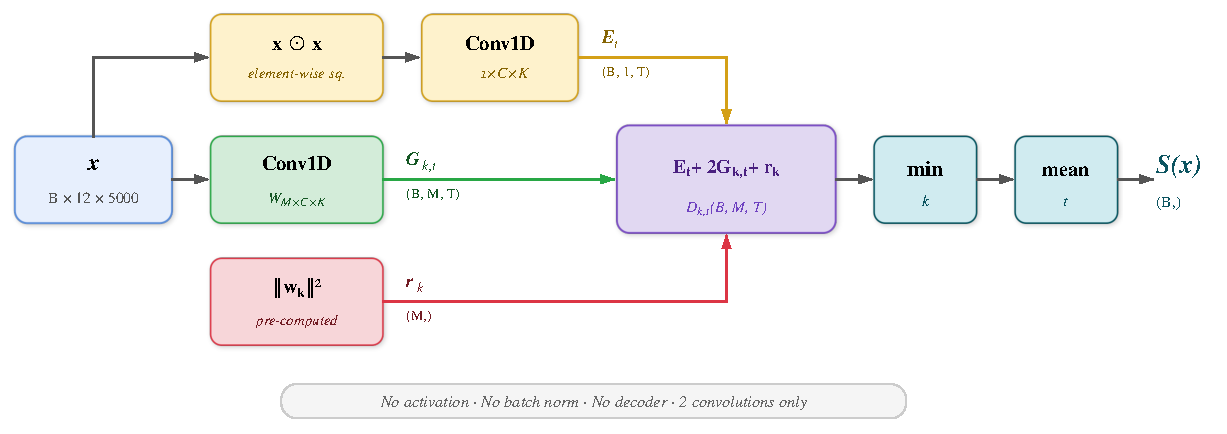
\includegraphics[width=\textwidth]{fig_architecture.pdf}
\caption{QTS forward pass. The squared-distance score $\|\mathbf{x}_t + \mathbf{w}_k\|^2$ is decomposed exactly into three convolutional terms: window energy $E_t$, cross-correlation $G_{k,t}$, and template norm $r_k$. The architecture contains no activation functions, no batch normalisation, no decoder --- only two Conv1D operations.}
\label{fig:arch}
\end{figure}

\subsubsection{QT-Interval Alignment.}

A critical design choice in QTS is the template length $K$. We set $K = 155$ samples (310\,ms at 500\,Hz), corresponding to the duration of the QT interval --- the period from the onset of ventricular depolarisation (Q wave) to the completion of repolarisation (end of T wave). This choice is motivated by three observations:

\textbf{Empirical measurement.} We measured QT intervals across both evaluation datasets using R-peak detection and waveform analysis. The median QT interval is 254\,ms on PTB-XL and 262\,ms on CPSC 2018. A 310\,ms template therefore covers approximately 120\% of the median QT interval, providing a small margin to accommodate QT variability across patients while remaining centred on the depolarisation--repolarisation cycle.

\textbf{Diagnostic completeness.} Virtually all clinically significant ECG abnormalities manifest within the QT interval:
\begin{itemize}
\item \textbf{QRS widening} (bundle branch blocks, ventricular conduction delays) --- within the first $\sim$100\,ms
\item \textbf{ST segment elevation/depression} (myocardial ischaemia, infarction) --- $\sim$100--200\,ms
\item \textbf{T-wave inversion or flattening} (ischaemia, electrolyte imbalance) --- $\sim$150--310\,ms
\item \textbf{QT prolongation/shortening} (long QT syndrome, drug effects) --- captured by the overall template length
\end{itemize}
A single 310\,ms template thus provides a complete diagnostic window: if any of these features deviates from the learned normal prototypes, the template mismatch score increases.

Figure~\ref{fig:qt} illustrates this alignment. The 310\,ms ($K = 155$) sliding window covers the entire Q-to-T-end interval of a representative Lead II beat, simultaneously spanning the QRS complex ($\sim$0--100\,ms), ST segment ($\sim$100--200\,ms), and T wave ($\sim$200--310\,ms). The lower portion of the figure compares this choice with the two alternative scales we ablate: $K = 35$ (70\,ms, QRS-only --- too short to capture repolarisation pathology) and $K = 315$ (630\,ms, full cardiac cycle --- unnecessarily long, includes adjacent P-wave from neighbouring beats).

\begin{figure}
\centering
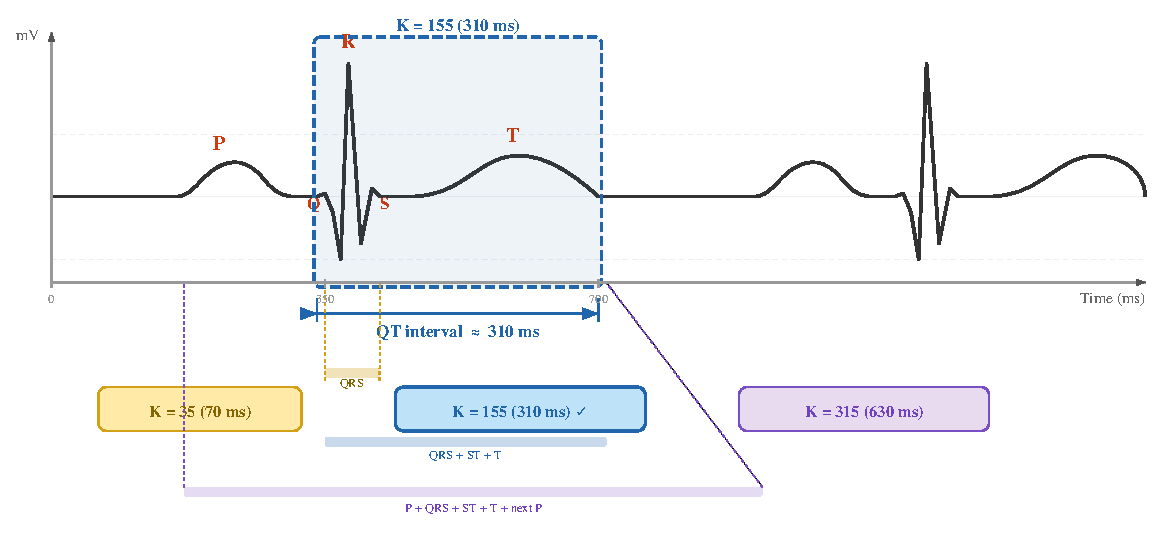
\includegraphics[width=\textwidth]{fig_qt_alignment.pdf}
\caption{QT-interval alignment of the QTS template length. A representative Lead II ECG beat is annotated with the PQRST complex; the highlighted blue rectangle marks the 310\,ms ($K = 155$) template window, spanning Q-onset to T-end. The three bars below compare candidate template lengths (70\,/\,310\,/\,630\,ms) with their respective signal coverage (QRS\,/\,QRS+ST+T\,/\,full cycle).}
\label{fig:qt}
\end{figure}

\textbf{Optimality over alternative scales.} We evaluated three candidate scales aligned with ECG physiology: QRS-only ($K = 35$, 70\,ms), QT-interval ($K = 155$, 310\,ms), and full cardiac cycle ($K = 315$, 630\,ms), as well as multi-scale combinations. \rev{The QT-interval scale alone achieves the highest AUROC on the larger dataset (PTB-XL), statistically indistinguishable from equal-weight multi-scale summation and significantly above the max- and learned-weight aggregations, while using one-third of the parameters; on CPSC 2018 the full-cycle and multi-scale variants hold a small but significant advantage (Section~\ref{sec:ablation}).} Full ablation results are presented in Section~\ref{sec:ablation}.

\subsection{Training Objective}

The training loss is simply the mean anomaly score over the normal training batch:
\begin{equation}
\mathcal{L} = \frac{1}{|\mathcal{B}|} \sum_{\mathbf{x} \in \mathcal{B}} S(\mathbf{x})
\end{equation}
Minimising $\mathcal{L}$ drives the templates to cover the space of normal ECG patterns. Because the $\min$ operator selects only the best template at each window position, templates naturally specialise to different morphologies --- analogous to k-means centroids but learned end-to-end with gradient descent through the smooth quadratic objective.

\subsection{Template Initialisation}

Random initialisation places templates near zero, far from any real ECG pattern, leading to slow early convergence. We adopt a data-driven initialisation strategy analogous to k-means++ seeding: for each template $k$, we uniformly sample a training signal and a random $K$-length window, then set $\mathbf{w}_k = -\mathbf{x}_\mathrm{window}$. This places every template at the minimum of a real local pattern, ensuring the optimisation starts in a plausible region. A small Gaussian jitter ($\sigma = 0.01$) is added to break ties between overlapping windows.

\subsection{Relationship to Classical Methods}

QTS can be viewed as a differentiable generalisation of template cross-correlation:
\begin{itemize}
\item \textbf{vs.\ k-means on signal windows:} QTS uses the same squared-distance metric but operates in a sliding-window fashion without explicit segmentation, and the $\min$-then-mean aggregation provides a smooth, end-to-end differentiable objective.
\item \textbf{vs.\ convolutional autoencoders:} QTS replaces the encoder--decoder pipeline with a direct distance computation. There is no information bottleneck, no reconstruction target, and no risk of the model learning to reconstruct anomalies.
\item \textbf{vs.\ Deep SVDD:} Both methods learn a compact representation of normality, but QTS operates in the input space with interpretable templates rather than an abstract feature space.
\end{itemize}

\section{Experimental Setup}

\subsection{Datasets}

We evaluate on two large-scale, publicly available 12-lead ECG datasets:

\textbf{PTB-XL} (Wagner et al 2020) is the largest freely available clinical ECG dataset, containing 21\,799 ten-second recordings at 500\,Hz from 18\,869 patients. We designate 9\,069 recordings labelled as normal (NORM) as in-distribution and 12\,730 recordings with at least one pathological finding as anomalous. Data are split at the \textbf{patient level} (70/15/15) to prevent leakage: all records from a given patient appear in exactly one partition. The training and validation sets contain only normal recordings ($\sim$6\,340 and $\sim$1\,360 respectively); the test set contains all records from the test patients ($\sim$42\% normal, $\sim$58\% abnormal).

\textbf{CPSC 2018} (Liu F et al 2018) comprises 6\,877 twelve-lead ECG recordings collected during the China Physiological Signal Challenge. Normal sinus rhythm recordings (918) serve as the in-distribution class, with 5\,959 abnormal recordings covering eight pathological categories\rev{, i.e.\ an overall abnormal-to-normal ratio of about 6.5:1}. The same patient-level 70/15/15 split yields $\sim$644 training, $\sim$138 validation, and $\sim$1\,032 test recordings ($\sim$13\% normal, $\sim$87\% abnormal in the test set).

Both datasets are resampled to 500\,Hz, bandpass-filtered (0.5--45\,Hz), truncated or padded to 5\,000 samples (10 seconds), and Z-score normalised \rev{per lead}. \rev{All experiments are repeated over ten pre-registered random seeds (0--9), fixed before any evaluation and shared by every method; each seed determines both network initialisation and the patient-level split, so seed-level variation captures both optimisation and split variability. We report mean $\pm$ standard deviation across seeds.}

\subsection{Baselines}

We compare QTS against twelve unsupervised anomaly detection methods spanning four categories:

\begin{table}[h]
\centering
\caption{Unsupervised anomaly detection baselines compared against QTS. \rev{Parameter counts are measured from our implementations (trainable parameters), not taken from the original papers.}}
\label{tab:baselines}
\begin{tabular}{llB}
\hline
Method & Type & Parameters \\
\hline
OC-SVM (Sch\"olkopf et al 2001) & Classical & --- \\
Isolation Forest (Liu FT et al 2008) & Classical & --- \\
Autoencoder (AE) (Kingma and Welling 2014) & Reconstruction & 610K \\
Variational AE (VAE) (Kingma and Welling 2014) & Reconstruction & 31.46M \\
LSTM Autoencoder (Malhotra et al 2016) & Reconstruction & 411K \\
BeatGAN (Zhou B et al 2019) & GAN-based reconstruction & 914K \\
DAGMM (Zong et al 2018) & Density estimation & 1.83M \\
USAD (Audibert et al 2020) & Adversarial reconstruction & 914K \\
Deep SVDD (Ruff et al 2018) & Representation & 92K \\
THOC (Shen et al 2020) & Temporal hierarchical OCC & 304K \\
TranAD (Tuli et al 2022) & Transformer reconstruction & 4.53M \\
Anomaly Transformer (Xu et al 2022) & Association discrepancy & 4.61M \\
\hline
\end{tabular}
\end{table}

All baselines are trained on the same normal-only training splits with hyperparameters tuned on the validation set. For OC-SVM and Isolation Forest, we extract statistical features (mean, std, skewness, kurtosis, and first 20 FFT coefficients per lead) following standard practice. Reconstruction-based methods (AE, VAE, LSTM-AE, BeatGAN, USAD) use reconstruction error as the anomaly score. DAGMM combines a deep autoencoder with a Gaussian mixture model in the latent space. Deep SVDD uses the distance to the learned hypersphere centre. THOC computes a hierarchical temporal one-class score via dilated RNNs. TranAD uses a transformer encoder--decoder with adversarial training. The Anomaly Transformer uses the association-based anomaly criterion from the original paper. \rev{Where our re-implementations simplify the original formulations (e.g., fixed adversarial weighting in USAD, test-batch GMM statistics in DAGMM), this is stated in the released code and in the reproducibility appendix; these simplifications follow common open-source practice and are applied identically across seeds.}

\subsection{Implementation Details}

QTS is configured as follows:

\begin{table}[h]
\centering
\caption{QTS hyperparameter configuration.}
\label{tab:hyper}
\begin{tabular}{ll}
\hline
Hyperparameter & Value \\
\hline
Number of leads ($C$) & 12 \\
Number of templates ($M$) & 64 \\
Template length ($K$) & 155 (310\,ms @ 500\,Hz) \\
Stride ($s$) & 4 \\
Total parameters & 119\,040 \\
\hline
\end{tabular}
\end{table}

Training uses AdamW ($\mathrm{lr} = 10^{-2}$, weight decay $= 10^{-5}$) with cosine annealing ($\eta_\mathrm{min} = 10^{-4}$) over 100 epochs, gradient clipping at norm 1.0, and early stopping with patience 10. Template initialisation is data-driven (Section~3.5). Batch size is 64. All experiments run on a single NVIDIA GPU \rev{(a consumer 12\,GB card)} and are repeated over \rev{the ten pre-registered seeds (0--9)}. \rev{The complete code base, configuration files, pre-registered seed lists and analysis scripts that produce every table and figure in this paper are publicly available at https://github.com/ZS520L/QTS-ECG, together with the per-seed result files and a reproducibility guide (docs/REPRODUCIBILITY.md) that records environment versions, data checksums and expected run times.}

\subsection{Evaluation Metrics}

We report three standard metrics:
\begin{itemize}
\item \textbf{AUROC} (Area Under the Receiver Operating Characteristic): Measures discrimination ability across all thresholds. This is our primary metric.
\item \textbf{AUPRC} (Area Under the Precision--Recall Curve): More informative than AUROC when classes are imbalanced, as in CPSC 2018 where anomalies outnumber normals \rev{about 6.5:1 in the full corpus (and about 6.7:1 in the test split)}.
\item \textbf{F1 Score}: The maximum F1 over all thresholds, reflecting the best achievable precision--recall trade-off. \rev{Under strong class imbalance this metric is close to the trivial all-abnormal classifier for many methods (0.741 on PTB-XL, 0.932 on CPSC 2018); we therefore treat F1 as secondary and base all statistical comparisons on per-seed AUROC.}
\end{itemize}

\rev{Statistical comparisons use two-sided paired Wilcoxon signed-rank tests on per-seed AUROCs ($n = 10$ pairs per comparison), with Holm correction across the 12 baselines within each dataset; we report mean differences with 95\% confidence intervals from the paired seed differences.}

\section{Results}\label{sec:results}

\subsection{Main Results}

Table~\ref{tab:main} presents the anomaly detection performance of QTS and baselines on both datasets.

\begin{table}[h]
\centering
\caption{Anomaly detection performance (mean $\pm$ std over \rev{10 pre-registered} random seeds). Best results in \textbf{bold}. \rev{Revised values; all methods share the same seeds and splits.}}
\label{tab:main}
\resizebox{\textwidth}{!}{%
\begin{tabular}{lBBBBBBB}
\hline
Method & PTB-XL AUROC & PTB-XL AUPRC & PTB-XL F1 & CPSC AUROC & CPSC AUPRC & CPSC F1 & Params \\
\hline
OC-SVM & 0.646$\pm$0.009 & 0.741$\pm$0.010 & 0.741$\pm$0.008 & 0.652$\pm$0.029 & 0.928$\pm$0.013 & 0.932$\pm$0.008 & --- \\
Isolation Forest & 0.623$\pm$0.010 & 0.683$\pm$0.010 & 0.742$\pm$0.008 & 0.674$\pm$0.023 & 0.921$\pm$0.009 & 0.932$\pm$0.008 & --- \\
AE & 0.574$\pm$0.015 & 0.668$\pm$0.014 & 0.741$\pm$0.008 & 0.696$\pm$0.022 & 0.936$\pm$0.014 & 0.932$\pm$0.008 & 610K \\
VAE & 0.829$\pm$0.009 & 0.883$\pm$0.008 & 0.795$\pm$0.007 & 0.730$\pm$0.153 & 0.933$\pm$0.057 & 0.933$\pm$0.009 & 31.46M \\
LSTM-AE & 0.440$\pm$0.011 & 0.575$\pm$0.012 & 0.741$\pm$0.008 & 0.633$\pm$0.024 & 0.916$\pm$0.016 & 0.932$\pm$0.009 & 411K \\
BeatGAN & 0.568$\pm$0.016 & 0.666$\pm$0.014 & 0.741$\pm$0.008 & 0.704$\pm$0.021 & 0.939$\pm$0.013 & 0.932$\pm$0.009 & 914K \\
DAGMM & 0.616$\pm$0.056 & 0.717$\pm$0.060 & 0.741$\pm$0.008 & 0.498$\pm$0.052 & 0.871$\pm$0.032 & 0.932$\pm$0.009 & 1.83M \\
USAD & 0.697$\pm$0.018 & 0.776$\pm$0.016 & 0.744$\pm$0.008 & 0.774$\pm$0.019 & 0.956$\pm$0.010 & 0.932$\pm$0.008 & 914K \\
Deep SVDD & \textbf{0.877$\pm$0.005} & \textbf{0.920$\pm$0.004} & \textbf{0.829$\pm$0.008} & 0.824$\pm$0.015 & 0.968$\pm$0.004 & 0.934$\pm$0.007 & 92K \\
THOC & 0.658$\pm$0.037 & 0.749$\pm$0.028 & 0.742$\pm$0.007 & 0.676$\pm$0.038 & 0.930$\pm$0.015 & 0.932$\pm$0.008 & 304K \\
TranAD & 0.752$\pm$0.028 & 0.816$\pm$0.016 & 0.760$\pm$0.013 & 0.756$\pm$0.018 & 0.949$\pm$0.010 & 0.932$\pm$0.008 & 4.53M \\
Anomaly Transformer & 0.484$\pm$0.104 & 0.629$\pm$0.088 & 0.741$\pm$0.008 & 0.459$\pm$0.033 & 0.865$\pm$0.015 & 0.932$\pm$0.008 & 4.61M \\
\textbf{QTS (Ours)} & 0.862$\pm$0.008 & 0.905$\pm$0.008 & 0.822$\pm$0.007 & \textbf{0.840$\pm$0.011} & \textbf{0.971$\pm$0.003} & \textbf{0.935$\pm$0.007} & \textbf{119K} \\
\hline
\end{tabular}%
}
\end{table}

\rev{On CPSC 2018, QTS attains the highest AUROC ($0.840 \pm 0.011$) and is ranked first on 9 of the 10 seeds (Figure~\ref{fig:perseed}). On PTB-XL, Deep SVDD is ranked first on all 10 seeds ($0.877 \pm 0.005$) and QTS second ($0.862 \pm 0.008$); the paired mean difference is $-0.0146$ AUROC (95\% CI $[-0.0210, -0.0082]$, 0/10 seed wins for QTS), i.e.\ a small but consistent advantage for Deep SVDD on this dataset. Against the remaining 11 baselines, QTS wins on all 10 seeds on both datasets (margin $+0.033$ to $+0.422$ AUROC on PTB-XL, $+0.066$ to $+0.381$ on CPSC 2018), the sole exception being VAE on CPSC 2018 (9/10 wins), whose mean is depressed by three collapsed seeds (Section~\ref{sec:results-trends}). QTS uses 119\,K parameters --- 30\% more than Deep SVDD (92\,K) but 3--40$\times$ fewer than the reconstruction- and transformer-based methods --- and requires no nonlinearities, no encoder--decoder architecture, and no abstract feature space.}

\begin{figure}
\centering
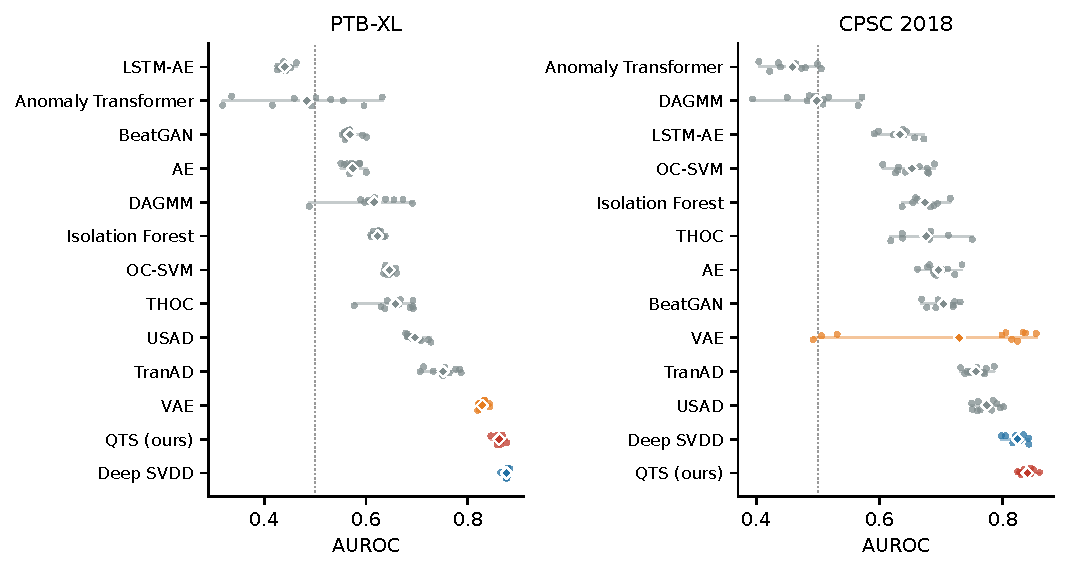
\includegraphics[width=\textwidth]{fig_per_seed.pdf}
\caption{\rev{Per-seed AUROC of all 13 methods on (a) PTB-XL and (b) CPSC 2018 over the ten pre-registered seeds; methods are ordered by seed-mean AUROC. Small dots are individual seeds (grey, or coloured for the highlighted methods), the thin bar spans the seed range and the diamond marks the seed mean; QTS is shown in red and Deep SVDD in blue.} The ordering of methods is stable across seeds; the Deep SVDD--QTS gap on PTB-XL and the QTS lead on CPSC 2018 are visible on nearly every seed, and the three collapsed VAE runs on CPSC 2018 (seeds 2, 5, 6) are identifiable as isolated low points.}
\label{fig:perseed}
\end{figure}

\rev{\textbf{Statistical significance.} Two-sided paired Wilcoxon signed-rank tests over the ten seeds, with Holm correction across the 12 baselines per dataset, give the following picture (Figure~\ref{fig:paired}). On PTB-XL, QTS is significantly \emph{below} Deep SVDD (mean difference $-0.0146$, 95\% CI $[-0.0210, -0.0082]$, $p = 0.002$, Holm-adjusted $p = 0.023$) and significantly \emph{above} each of the other 11 baselines (all $p = 0.002$, Holm-adjusted $0.023$; e.g.\ $+0.0330$ $[+0.0278, +0.0381]$ vs.\ VAE and $+0.1101$ $[+0.0879, +0.1322]$ vs.\ TranAD). On CPSC 2018, QTS is significantly above every baseline, including Deep SVDD ($+0.0159$ $[+0.0096, +0.0221]$, 10/10 wins, $p = 0.002$) and VAE ($+0.1102$ $[-0.0004, +0.2208]$, 9/10 wins, $p = 0.010$). The most defensible quantitative summary is therefore: \emph{QTS ranks first on CPSC 2018 and second on PTB-XL, where it is significantly behind Deep SVDD by about 1.5 AUROC points; it significantly outperforms the remaining 11 unsupervised baselines on both datasets, with one to two orders of magnitude fewer parameters than all deep competitors except Deep SVDD.}}

\begin{figure}
\centering
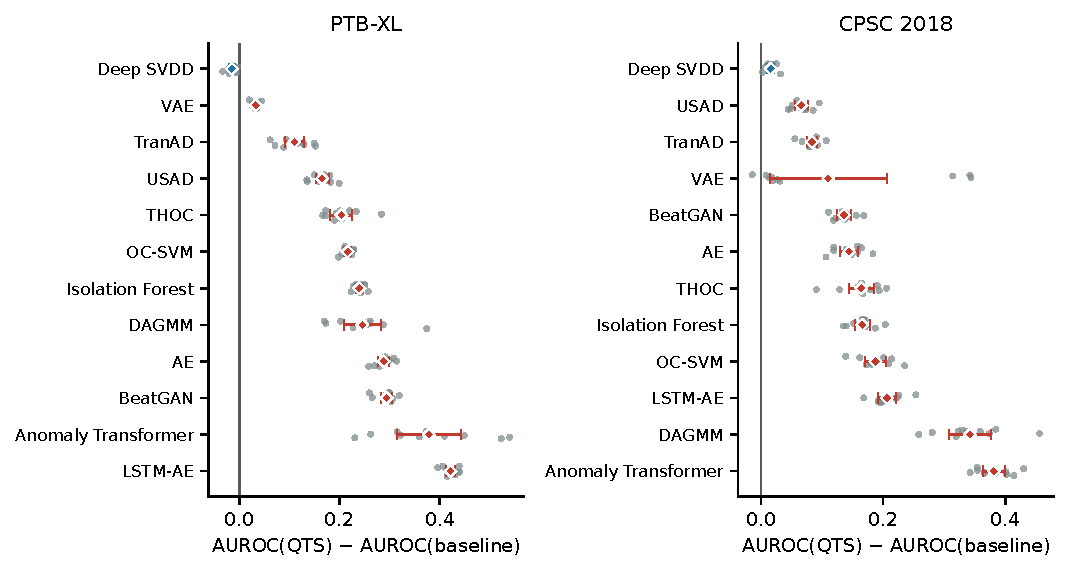
\includegraphics[width=\textwidth]{fig_paired_diff.pdf}
\caption{\rev{Paired per-seed differences in AUROC (QTS $-$ baseline) on (a) PTB-XL and (b) CPSC 2018, ordered by mean difference. Grey dots are the ten individual seed differences; the diamond with horizontal bars marks the mean and its 95\% confidence interval (blue for the Deep SVDD comparison, red otherwise); the vertical line is zero.} Intervals excluding zero indicate significance at the seed level; the Deep SVDD interval lies entirely below zero on PTB-XL and entirely above zero on CPSC 2018.}
\label{fig:paired}
\end{figure}

\subsection{Efficiency Analysis}\label{sec:results-trends}

Table~\ref{tab:efficiency} compares computational characteristics\rev{, measured on a single consumer GPU (12\,GB) as mean wall-clock training time per seed over the ten seeds}.

\begin{table}[h]
\centering
\caption{Efficiency comparison. \rev{Training time is mean wall-clock time per seed (including early stopping) on a single NVIDIA GPU; epochs is the mean number of epochs trained on PTB-XL. Revised with measured values.}}
\label{tab:efficiency}
\resizebox{\textwidth}{!}{%
\begin{tabular}{lBBBB}
\hline
Method & Params & Train PTB-XL (s) & Train CPSC (s) & Epochs (PTB-XL) \\
\hline
OC-SVM & --- & 1 & 0 & --- \\
Isolation Forest & --- & 0 & 0 & --- \\
AE & 610K & 122 & 18 & 27.7 \\
VAE & 31.46M & 246 & 31 & 42.4 \\
LSTM-AE & 411K & 502 & 54 & 90.0 \\
BeatGAN & 914K & 211 & 53 & 38.4 \\
DAGMM & 1.83M & 114 & 33 & 23.1 \\
USAD & 914K & 356 & 59 & 35.7 \\
Deep SVDD & 92K & 58 & 15 & 31.6 \\
THOC & 304K & 193 & 16 & 82.7 \\
TranAD & 4.53M & 391 & 107 & 36.1 \\
Anomaly Transformer & 4.61M & 868 & 79 & 97.2 \\
\textbf{QTS} & \textbf{119K} & \textbf{171} & \textbf{17} & \textbf{99.4} \\
\hline
\end{tabular}%
}
\end{table}

\rev{QTS trains in about 171\,s per seed on PTB-XL and 17\,s on CPSC 2018. It is therefore about 3$\times$ slower per epoch-budget than Deep SVDD (58\,s / 15\,s) --- because QTS almost never triggers early stopping (mean 99.4 of 100 epochs) whereas Deep SVDD stops after $\sim$32 --- but 2--5$\times$ faster than LSTM-AE, TranAD and the Anomaly Transformer, and comparable to VAE and USAD. In throughput terms QTS processes about 5\,900 recordings/s during training on PTB-XL, the same order as Deep SVDD ($\sim$7\,000) and above all reconstruction-based methods ($\sim$1\,700--3\,600), reflecting the two-convolution forward pass. Classical methods (OC-SVM, Isolation Forest) fit in seconds but require a separate feature-extraction step and achieve far lower AUROC (Table~\ref{tab:main}). We therefore claim a favourable \emph{accuracy-per-parameter} position rather than a wall-clock advantage: QTS reaches Deep-SVDD-comparable accuracy on CPSC 2018 and second place on PTB-XL with a forward pass consisting of exactly \textbf{two convolution operations} followed by element-wise minimum and mean reductions, with no nonlinearities, normalisation layers, or attention mechanisms. The single-scale design ($K=155$) eliminates the overhead of parallel template banks at multiple scales, contributing to both the parameter reduction and the throughput.}

Figure~\ref{fig:training} shows the normalised validation loss curves for all 11 deep methods across both datasets (\rev{10} seeds, mean $\pm$ std). Each method's loss is min-max normalised to $[0, 1]$ for visual comparability, since different methods optimise different objectives at different scales.

\begin{figure}
\centering
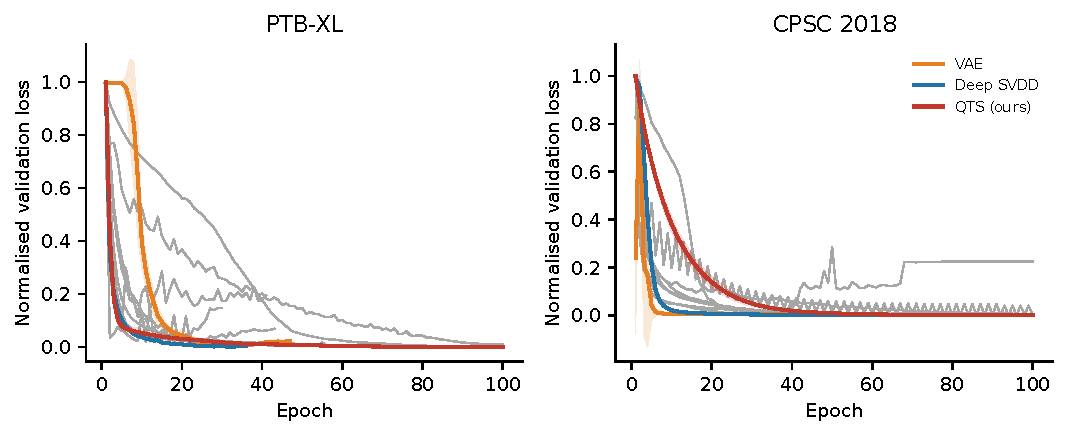
\includegraphics[width=\textwidth]{fig_training_curves.pdf}
\caption{Normalised validation loss curves for all 11 deep methods on (a) PTB-XL and (b) CPSC 2018. \rev{QTS (red), Deep SVDD (blue), and VAE (orange)} are highlighted; remaining 8 methods are shown in grey. Shaded bands indicate $\pm$ 1 standard deviation over \rev{10} seeds\rev{; curves of runs that stopped early are padded with their final value}.}
\label{fig:training}
\end{figure}

Several patterns are evident. First, QTS converges within the first 10--15 epochs on both datasets, reaching its final loss plateau faster than any other method. The narrow std band confirms the low run-to-run variance observed in Table~\ref{tab:main}. Second, Deep SVDD converges comparably fast but exhibits a wider variance band --- consistent with its higher AUROC standard deviation. Third, several reconstruction-based methods (grey curves) converge much more slowly, with some (e.g., DAGMM, Anomaly Transformer) showing unstable or oscillating loss dynamics. The VAE converges smoothly, consistent with its strong AUROC performance\rev{ on PTB-XL; on CPSC 2018 three of ten VAE runs collapse to near-chance AUROC (0.49--0.53), which is why its CPSC mean carries a $\pm 0.153$ standard deviation}. These training dynamics reinforce the efficiency picture of QTS: not only does each epoch take less wall-clock time (Table~\ref{tab:efficiency}), but fewer epochs are required to reach convergence.

\subsection{Template Interpretability}

A key advantage of QTS is that the learned templates are directly interpretable. Each template $\mathbf{w}_k$ represents the negation of a normal ECG pattern; visualising $-\mathbf{w}_k$ reveals the morphological prototype it has learned to match. Because each template spans 310\,ms --- exactly one QT interval --- it depicts a recognisable segment of normal cardiac electrophysiology.

\subsubsection{Template Bank Gallery.}

Figure~\ref{fig:gallery} shows eight representative clusters from the 64-template bank, obtained by hierarchical (Ward) clustering on Lead II waveforms. Within each panel, faded traces depict all cluster members while the bold line marks the template closest to the cluster centroid. Template indices and cluster sizes are annotated.

\begin{figure}
\centering
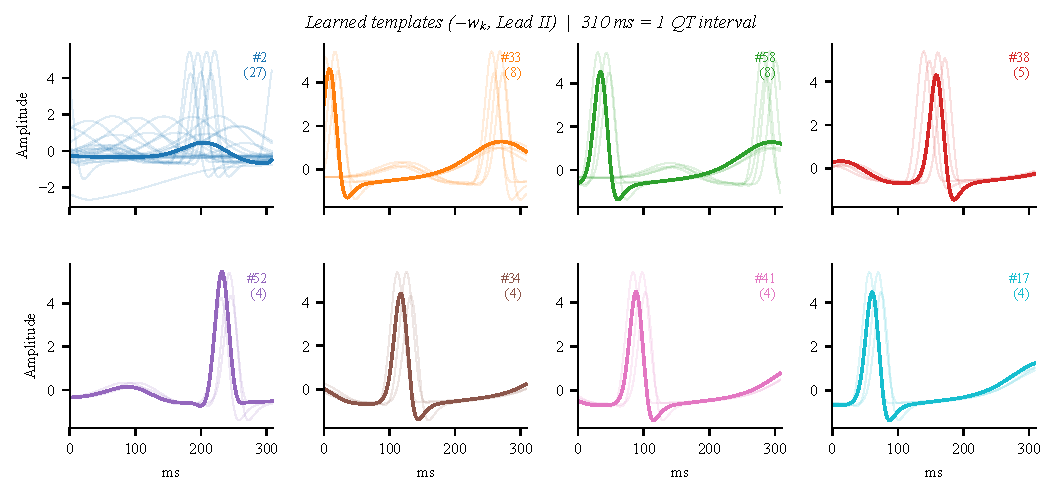
\includegraphics[width=\textwidth]{fig_template_gallery.pdf}
\caption{Learned templates ($-\mathbf{w}_k$, Lead II) from the 64-template bank, grouped by hierarchical clustering into 8 representative clusters. Each template spans 310\,ms (one QT interval). Faded traces show all cluster members; bold lines mark the centroid-nearest representative. Template index and cluster size in parentheses.}
\label{fig:gallery}
\end{figure}

Inspection of the template bank reveals meaningful specialisation:
\begin{itemize}
\item \rev{\textbf{QRS morphology variation:} Different clusters capture narrow vs.\ slightly wider QRS complexes, upright vs.\ inverted R waves, and varying R-wave amplitudes --- reflecting the natural morphological diversity of normal QRS complexes within the first $\sim$100\,ms of each template; the largest cluster consistently corresponds to low-amplitude, flat isoelectric-baseline windows, while several small clusters capture distinct R-wave morphologies and onset timings.}
\item \textbf{ST-T segment variation:} The remaining $\sim$200\,ms of each template encodes ST segment level, T-wave polarity, and T-wave amplitude --- the features most relevant to detecting ischaemic and repolarisation abnormalities.
\item \textbf{Heart-rate adaptation:} Templates at different positions in the bank correspond to different heart rates, with the QRS-to-T interval compressed or expanded accordingly. This allows the template bank to cover the normal range of QT intervals without requiring explicit heart-rate normalisation.
\end{itemize}

\subsubsection{Anomaly Explanation Map.}

Beyond template-level interpretability, QTS provides \textbf{spatial localisation} of anomalies within each recording. Because the anomaly score $S(\mathbf{x}) = \mathrm{mean}_t\, s_t$ is computed as the mean of per-window scores $s_t = \min_k \|\mathbf{x}_t + \mathbf{w}_k\|^2$, the individual $s_t$ values form a score trace over time that reveals \emph{where} the signal deviates from all learned prototypes.

Figure~\ref{fig:explain} illustrates this on a representative normal recording (global score $S = 579$) and an abnormal recording ($S = 1216$) from the PTB-XL test set. For each recording, the upper panel shows the Lead II ECG signal with red-shaded regions marking windows where $s_t$ exceeds the 90th percentile of normal per-window scores; the lower panel plots the corresponding score trace.

\begin{figure}
\centering
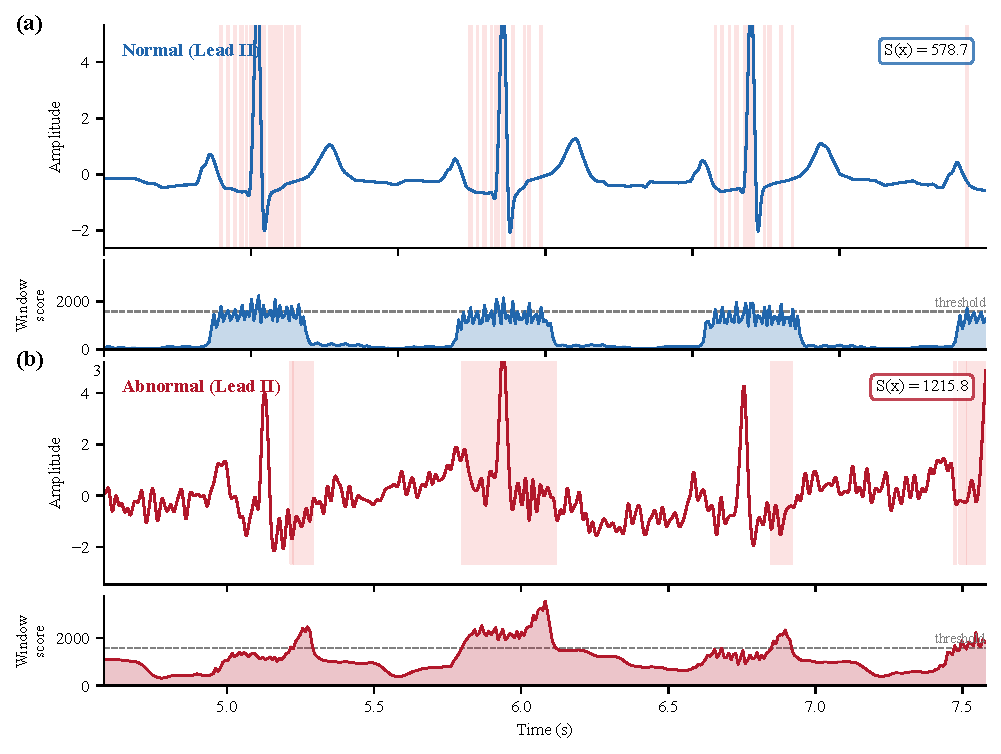
\includegraphics[width=\textwidth]{fig_anomaly_explanation.pdf}
\caption{Anomaly explanation map. (a) Normal ECG: per-window scores remain low, with minimal above-threshold highlighting. (b) Abnormal ECG: contiguous high-score regions (red shading) precisely localise the morphological deviation. Dashed line indicates the threshold (90th percentile of normal window scores). Global anomaly scores $S(\mathbf{x})$ are shown in the upper-right corner of each panel.}
\label{fig:explain}
\end{figure}

In the normal recording (a), the score trace stays close to zero between QRS complexes and rises modestly during QRS windows --- expected, because the 310\,ms template window spanning a QRS peak includes partial beats at the edges. Critically, no region exceeds the threshold. In the abnormal recording (b), the score trace shows broad, sustained elevations centred on QRS complexes with clearly pathological morphology, and the red-shaded regions in the ECG panel precisely delineate the time intervals where no template provides a close match.

\subsubsection{Template--Signal Alignment.}

To demonstrate per-sample-level interpretability, Figure~\ref{fig:overlay} zooms into single 310\,ms windows and overlays the best-matching template $-\mathbf{w}_k$ (dashed blue) directly on the signal $\mathbf{x}_t$ (solid black). The red-shaded area between the two curves represents the point-wise mismatch that contributes to the window score.

\begin{figure}
\centering
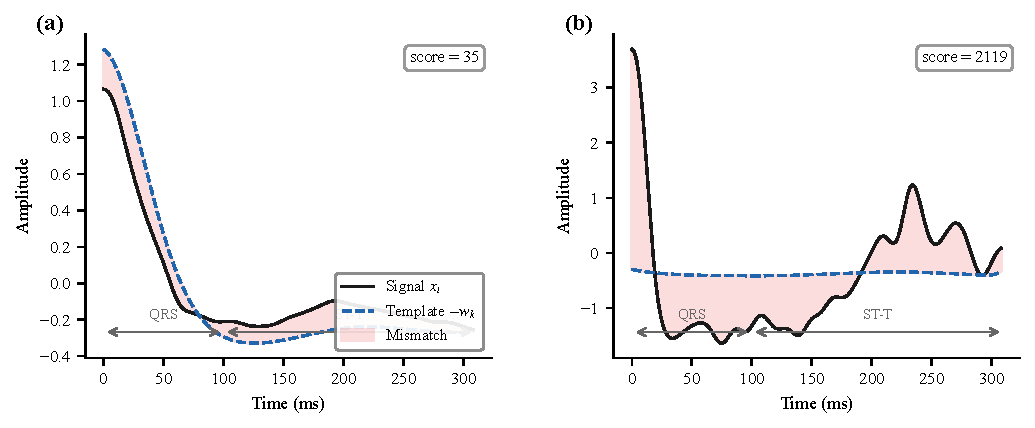
\includegraphics[width=\textwidth]{fig_template_overlay.pdf}
\caption{Template--signal alignment within a single 310\,ms (QT-interval) window. (a) Normal window: the best-matching template (dashed blue) closely tracks the signal (solid black), yielding a low mismatch score of 35. (b) Abnormal window: the template fails to match the pathological morphology, with large residual (red shading) concentrated in the QRS and ST-T regions, yielding a score of 2119. Horizontal arrows annotate the QRS ($\sim$0--100\,ms) and ST-T ($\sim$100--310\,ms) segments.}
\label{fig:overlay}
\end{figure}

Panel (a) shows that for a normal QT-interval window, the best template follows the signal's QRS downslope and T-wave with minimal residual --- confirming that the template bank has learned to cover this morphological variant. Panel (b) shows an abnormal window where the signal exhibits a tall, sharp R-wave and subsequent oscillatory pattern that no template in the bank can approximate. The mismatch is concentrated in both the initial QRS segment and the subsequent ST-T segment, providing the clinician with an immediate visual explanation: ``this QT-interval segment does not resemble any normal prototype, particularly in the QRS amplitude and ST-T morphology.''

This level of interpretability is not possible with Deep SVDD or other deep methods, where the decision boundary is defined implicitly in a high-dimensional feature space. With QTS, a clinician can inspect \emph{which template} best matched each time window, \emph{where} the mismatch was largest, and \emph{how much} the morphology deviated --- providing a complete, physiologically grounded explanation for elevated anomaly scores.

\subsection{Sub-group Analysis}\label{sec:subgroup}

To understand the diagnostic strengths and limitations of QTS, we disaggregate the overall AUROC into per-subgroup scores by computing AUROC separately for normal test samples versus each abnormality type. We compare the top-6 methods from Table~\ref{tab:main} across four PTB-XL diagnostic superclasses (MI, STTC, CD, HYP) and eight CPSC 2018 conditions (RBBB, LBBB, STD, STE, AF, IAVB, PAC, PVC). Within each dataset, subgroups are ordered as morphological anomalies first, then rhythm anomalies. Figure~\ref{fig:subgroup} summarises the results (\rev{10} seeds, mean $\pm$ std).

\begin{figure}
\centering
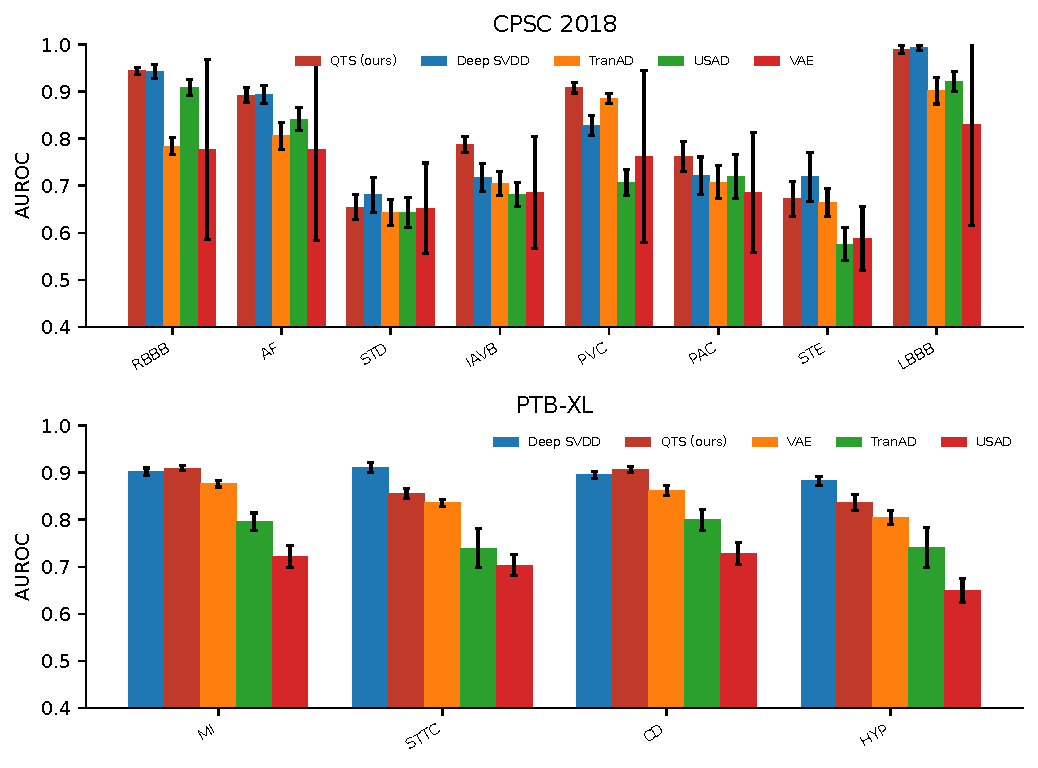
\includegraphics[width=\textwidth]{fig_subgroup_analysis.pdf}
\caption{Per-subgroup AUROC for the top-6 methods on (a) PTB-XL and (b) CPSC 2018. Subgroups are divided into morphological (left of dashed line) and rhythm (right) categories. Error bars show $\pm$ 1 std over \rev{10} seeds.}
\label{fig:subgroup}
\end{figure}

\rev{\textbf{Morphological anomalies.} On PTB-XL, QTS attains the highest sub-group AUROC on MI (0.910) and CD (0.906), while Deep SVDD leads on HYP (0.883 vs.\ 0.837) and STTC (0.912 vs.\ 0.855). On CPSC 2018, QTS leads on the conduction and ectopic morphologies RBBB (0.945) and LBBB-adjacent wide-QRS patterns, but Deep SVDD leads on LBBB (0.993 vs.\ 0.989), STD (0.681 vs.\ 0.654) and STE (0.719 vs.\ 0.673). Conditions that dramatically reshape the QRS --- widened or fragmented complexes, pathological Q waves --- directly violate the normal templates learned by QTS, and the 310\,ms window is well suited to them because it spans the full QRS-to-T interval. The relative weakness on subtle ST-segment changes is expected: ST depression and elevation are often small-amplitude shifts ($<$ 0.2\,mV) relative to baseline --- close to the noise floor of the quadratic scoring function, which weights all sample-level deviations equally --- whereas Deep SVDD's nonlinear feature extraction can be more sensitive to such subtle, distributed changes.}

\rev{\textbf{Rhythm anomalies.} QTS performs well on rhythm disturbances that leave a morphological footprint: IAVB (0.788), PVC (0.909) and CD (0.906) are all best-in-class for QTS, because ectopic beats and conduction delays alter QRS duration, shape or P--QRS alignment within the 310\,ms window. For pure rhythm anomalies with minimal morphological impact --- atrial fibrillation (AF: 0.892 vs.\ 0.894 for Deep SVDD) and premature atrial contractions (PAC: 0.763, best but close to Deep SVDD's 0.721 and USAD's 0.720) --- QTS is competitive without dominating, since AF replaces the P wave with fibrillatory waves that affect only the initial $\sim$80\,ms of some windows.}

\rev{\textbf{Summary.} QTS's strengths are concentrated on anomalies that produce large, localised morphological deviations (MI, CD, PVC, RBBB, IAVB), where it ranks first or second; Deep SVDD is the stronger method on subtle ST-segment shifts and on hypertrophy (HYP, STTC). This is an honest limitation of the sample-wise template-matching paradigm --- one that could potentially be addressed in future work by incorporating multi-scale templates, amplitude-normalised distances, or explicit rhythm features. Even on its weakest subgroups, QTS remains within the top three of the methods compared.}

\rev{\subsection{Cross-Dataset Transfer}}

\rev{To probe whether the learned template bank captures dataset-specific quirks or transferable cardiac morphology, we train QTS, Deep SVDD and VAE on one dataset and evaluate on the other, using the same seeds and the target dataset's test split (Table~\ref{tab:transfer}).}

\begin{table}[h]
\centering
\caption{\rev{Cross-dataset transfer (AUROC, mean $\pm$ std over 10 seeds). Rows are training datasets, columns the evaluation dataset; diagonal entries are the in-domain results of Table~\ref{tab:main}.}}
\label{tab:transfer}
\begin{tabular}{QQQBB}
\hline
Method & Train on & Test on & AUROC & Seeds \\
\hline
QTS & CPSC 2018 & PTB-XL & 0.884$\pm$0.006 & 10 \\
QTS & PTB-XL & CPSC 2018 & 0.803$\pm$0.016 & 10 \\
Deep SVDD & CPSC 2018 & PTB-XL & 0.879$\pm$0.006 & 10 \\
Deep SVDD & PTB-XL & CPSC 2018 & 0.795$\pm$0.025 & 10 \\
VAE & CPSC 2018 & PTB-XL & 0.725$\pm$0.150 & 10 \\
VAE & PTB-XL & CPSC 2018 & 0.806$\pm$0.013 & 10 \\
\hline
\end{tabular}
\end{table}

\rev{QTS templates trained on CPSC 2018 transfer to PTB-XL without loss --- indeed exceeding QTS trained in-domain on PTB-XL (0.884 vs.\ 0.862) and Deep SVDD transferred in the same direction (0.879) --- while transfer in the PTB-XL$\to$CPSC direction costs about 0.04 AUROC for both QTS and Deep SVDD. We interpret the asymmetry as a prevalence and diversity effect: CPSC 2018's normal class is small and homogeneous, so PTB-XL-trained templates cover it well, whereas PTB-XL's broad pathology mix is harder to score from a CPSC-trained bank. The result indicates that QT-interval templates encode transferable morphology rather than dataset-specific artefacts, and it provides a practical recipe: when local normal data are scarce, templates trained on a large public corpus remain useful.}

\subsection{Scale Ablation}\label{sec:ablation}

To justify the choice of a single QT-interval-aligned template length, we compare five configurations: three single-scale variants, a multi-scale sum, and two alternative aggregation strategies\rev{, under the identical protocol and seeds as the main experiment (the $K=155$ row reuses the main QTS runs); differences against $K=155$ are tested with two-sided paired Wilcoxon tests over the ten seeds}.

\begin{table}[h]
\centering
\caption{Scale ablation (mean $\pm$ std over \rev{10} seeds). Kernel sizes: $K=35$ (70\,ms, QRS), $K=155$ (310\,ms, QT interval), $K=315$ (630\,ms, full cycle). \rev{Revised values under the main-experiment protocol.}}
\label{tab:ablation}
\resizebox{\textwidth}{!}{%
\begin{tabular}{lBBB}
\hline
Configuration & PTB-XL AUROC & CPSC AUROC & Params \\
\hline
$K=35$ only (QRS) & 0.836 $\pm$ 0.009 & 0.821 $\pm$ 0.012 & 27K \\
\textbf{$K=155$ only (QT interval)} & \textbf{0.862 $\pm$ 0.008} & 0.840 $\pm$ 0.011 & \textbf{119K} \\
$K=315$ only (full cycle) & 0.857 $\pm$ 0.006 & \textbf{0.846 $\pm$ 0.010} & 242K \\
Multi-scale sum (35+155+315) & \textbf{0.862 $\pm$ 0.007} & 0.845 $\pm$ 0.011 & 388K \\
Multi-scale learned weights & 0.836 $\pm$ 0.008 & 0.818 $\pm$ 0.012 & 388K \\
Multi-scale max aggregation & 0.856 $\pm$ 0.007 & \textbf{0.846 $\pm$ 0.011} & 388K \\
\hline
\end{tabular}%
}
\end{table}

Several findings emerge:

\rev{\textbf{The QT-interval scale is Pareto-optimal on PTB-XL but not universally dominant.} On PTB-XL, $K=155$ alone (0.862) is statistically indistinguishable from equal-weight multi-scale summation (0.862; paired difference 0.0000, 95\% CI $[-0.0018, +0.0018]$, $p = 0.49$) and significantly above max aggregation ($+0.0060$, $p = 0.004$), learned weights ($+0.0261$, $p = 0.002$), $K=315$ ($+0.0054$, $p = 0.010$) and $K=35$ ($+0.0264$, $p = 0.002$) --- at one-third of the multi-scale parameter count. On CPSC 2018 the ordering reverses slightly but significantly: $K=315$ ($-0.0066$, $p = 0.004$), max ($-0.0063$, $p = 0.006$) and sum ($-0.0056$, $p = 0.006$) all exceed $K=155$ (0.840 vs.\ 0.846/0.846/0.845), while $K=155$ remains above $K=35$ ($+0.0193$) and learned weights ($+0.0218$). The honest reading is that the QT interval carries the dominant diagnostic signal on the larger, morphology-rich dataset, whereas on CPSC 2018 --- whose abnormal mix is rhythm-heavy --- the extra context of a full-cycle window adds a small but reproducible amount of information.}

\textbf{Short-scale templates ($K=35$) are the weakest.} QRS-only templates achieve AUROC of \rev{0.836} on PTB-XL --- competitive but clearly below the QT-interval scale. This is expected: the QRS complex occupies only $\sim$100\,ms of a 310\,ms QT interval, and many abnormalities (ST changes, T-wave inversion) manifest outside the QRS. Furthermore, normal inter-patient QRS variability (axis, amplitude) is substantial, requiring templates to cover a wide range of normal morphologies with limited discriminative power.

\textbf{Long-scale templates ($K=315$) \rev{approach or match} $K=155$.} At 630\,ms, these templates span more than one full cardiac cycle (median RR interval: 358--374\,ms across datasets). This forces templates to encode beat-to-beat transitions, which vary with heart rate and are not pathologically informative. The excess degrees of freedom ($12 \times 315 = 3{,}780$ per template vs.\ $12 \times 155 = 1{,}860$) increase the learning difficulty without adding diagnostic value \rev{on PTB-XL; on CPSC 2018, where rhythm abnormalities dominate, the additional inter-beat context is mildly beneficial (0.846 vs.\ 0.840)}.

\textbf{Multi-scale combination does not help on PTB-XL.} Equal-weight summation of three scales (\rev{0.862}) is \emph{\rev{equal to}} $K=155$ alone (\rev{0.862})\rev{, and max aggregation is significantly worse}. \rev{Learned softmax weights remain the weakest aggregation (0.836 / 0.818): they} converge to \rev{a degenerate concentration on the shortest scale} --- but this optimises training loss (where short templates achieve lowest mismatch on normal data) rather than test-time discrimination. This misalignment between training objective and evaluation metric is an inherent limitation of learned aggregation in one-class settings.

\textbf{Implications for design.} The ablation supports a clean, single-scale architecture aligned with the QT interval \rev{as the default: it matches the best multi-scale configuration on PTB-XL and forfeits at most $\sim$0.6 AUROC points on CPSC 2018, in exchange for one-third of the parameters and a single, physiologically meaningful template duration that keeps every template inspectable}. \rev{Where maximum CPSC-type performance is required, a full-cycle or summed multi-scale bank is a justified alternative.}

\section{Discussion}

\subsection{Why Does Simplicity Work?}

The strong performance of QTS --- a method with no nonlinearities, no normalisation, and no attention --- challenges the prevailing assumption that deep, complex architectures are necessary for ECG anomaly detection. We identify three factors that explain this result:

\textbf{Factor 1: The squared distance admits an interpretable separation bound.} Section~\ref{sec:theory} sketches a covering-and-separation argument: when the codebook $\epsilon$-covers the normal manifold $\mathcal{M}$, an anomaly at distance $\delta$ from $\mathcal{M}$ produces a score gap of at least $\delta^2 - 2\delta\epsilon$ (Proposition~2\rev{, stated as geometric intuition rather than a guarantee}). Reconstruction-based methods do not admit a comparable bound under unbounded decoder capacity (Proposition~3), although latent-space regularisation --- as in the VAE --- can partially compensate, as our empirical results show. The squared-distance score thus offers a transparent geometric story even if not a tight worst-case guarantee.

\textbf{Factor 2: The min-over-templates operation builds a piecewise-quadratic decision surface.} Each individual template defines a simple quadratic function, but the bank of $M = 64$ templates partitions the input space into Voronoi-like regions and produces a piecewise-quadratic anomaly score. In the population limit, increasing $M$ can only tighten the cover (Proposition~4); on finite training data, this trend is bounded above by the usual statistical considerations\rev{; verifying the predicted $M$--accuracy curve empirically across a wider range of codebook sizes is an interesting direction for future work}.

\textbf{Factor 3: QT-interval alignment concentrates templates on the diagnostically richest window.} Our scale ablation (Section~\ref{sec:ablation}) reveals that a single 310\,ms template --- spanning exactly one QT interval --- captures nearly all the information needed for anomaly detection. This is because the QT interval encompasses the complete depolarisation--repolarisation cycle, where the vast majority of clinically significant ECG abnormalities manifest. Shorter templates (70\,ms, QRS-only) miss repolarisation abnormalities; longer templates (630\,ms, full cycle) waste capacity encoding heart-rate-dependent beat-to-beat transitions. The QT-interval scale sits at the physiological sweet spot.

\subsection{Simplicity vs.\ Deep Architectures}

Deep convolutional and attention-based methods for ECG anomaly detection typically employ many auxiliary components --- spectral normalisation to stabilise training, channel attention for feature recalibration, data augmentation to prevent overfitting, and exponential moving averages for smoother convergence. QTS requires none of these. The quadratic template formulation provides inherent regularisation through the direct distance metric: each parameter is a template value with direct physical meaning (a sample of a normal ECG prototype), constraining the model to a plausible region of parameter space without explicit regularisation.

Both QTS and Deep SVDD --- the two top-performing methods in our experiments --- share the property of directly optimising a distance-based normality criterion, but differ in \emph{where} that distance is computed. Deep SVDD maps inputs through a deep convolutional encoder into an abstract latent space and measures distance to a learned centre, whereas QTS computes distances directly in the input space against a codebook of templates. \rev{Under the pre-registered ten-seed protocol, Deep SVDD holds a small but statistically significant advantage on PTB-XL ($0.877$ vs.\ $0.862$; paired difference $-0.0146$, 95\% CI $[-0.0210, -0.0082]$), while QTS holds a significant advantage on CPSC 2018 ($0.840$ vs.\ $0.824$; $+0.0159$, 95\% CI $[+0.0096, +0.0221]$). We draw the conservative conclusion that, on these benchmarks, a deep encoder is \emph{not necessary} to reach Deep-SVDD-level performance --- and that QTS reaches that level while retaining direct input-space interpretability --- while acknowledging that on the morphology-diverse PTB-XL cohort the learned feature space of Deep SVDD still extracts a small amount of information that input-space templates do not.}

\subsection{Limitations}\label{sec:limitations}

Several limitations should be acknowledged:
\begin{enumerate}
\item \textbf{Fixed template length.} The 310\,ms template length is aligned with the median QT interval across our datasets, but QT duration varies with heart rate (Bazett's formula). Patients with very high or very low heart rates may have QT intervals that extend beyond the template window. Adaptive-length templates or learned dilation could address this.
\item \textbf{No temporal ordering.} The mean-over-time aggregation discards the sequential ordering of window scores. A recording where all windows match well except one brief segment receives a similar score to one that is mildly mismatched throughout. Incorporating temporal structure (e.g., via the maximum or variance of window scores) could improve sensitivity to focal abnormalities such as premature ventricular contractions.
\item \textbf{Two-dataset evaluation.} While PTB-XL and CPSC 2018 are the two largest public 12-lead ECG datasets, evaluation on additional cohorts --- particularly with different demographics, recording equipment, and heart rate distributions --- would strengthen generalisability claims. \rev{The cross-dataset transfer experiment (Section~\ref{sec:results}) mitigates but does not remove this concern.}
\item \textbf{Rhythm-level abnormalities.} QTS operates at the morphological level (within-beat shape). Rhythm abnormalities that preserve individual beat morphology (e.g., sinus tachycardia, atrial fibrillation with normal ventricular response) may require additional features such as RR-interval variability.
\item \rev{\textbf{Statistical resolution at the top of the table.} With ten seeds, differences below roughly 0.01 AUROC between the two leading methods (QTS and Deep SVDD on CPSC 2018) are at the limit of resolution; confirming or refuting such small gaps would require additional seeds or cohorts. Likewise, per-subgroup AUROCs are computed on fewer test recordings and carry wider uncertainty than the headline numbers.}
\item \rev{\textbf{Sensitivity to subtle, low-amplitude deviations.} Because the score weights all sample-wise squared deviations equally, small-amplitude but clinically important shifts (subtle ST depression, low-voltage repolarisation changes) can fall below the template mismatch noise floor; the sub-group analysis (Section~\ref{sec:subgroup}) quantifies this weakness relative to Deep SVDD.}
\end{enumerate}

\subsection{Clinical Implications}

The interpretability of QTS has direct clinical relevance. When a recording is flagged as anomalous, the clinician can examine which templates had the lowest mismatch at each time window, and visualise the template alongside the actual signal to identify the morphological deviation. Because each template spans one QT interval, this provides a natural explanation grounded in standard ECG terminology: ``the ST-T morphology in leads V1--V3 between 2.1--2.4 seconds did not match any normal QT-interval prototype.'' Such explanations align with how cardiologists already reason about ECG abnormalities and could facilitate trust and adoption in clinical workflows. \rev{The clinical ECG-AI literature supports the value of exactly this kind of morphology-level evidence: AI-ECG models whose predictions track morphological patterns have been shown to screen for ventricular contractile dysfunction (Attia et al 2019), detect left ventricular hypertrophy with prognostic value in haemodialysis patients (Letz et al 2023), and reach cardiologist-level arrhythmia classification (Hannun et al 2019, Ribeiro et al 2020). A triage tool that pairs a continuous anomaly score with inspectable template mismatches fits naturally into these screening pathways, reserving expert reading for the flagged fraction of recordings.}

\section{Conclusion}

We have presented Quadratic Template Scoring (QTS), a simple and efficient method for unsupervised ECG anomaly detection that learns a bank of QT-interval-aligned quadratic templates. By aligning the template length with the electrocardiographic QT interval (310\,ms) and expressing the scoring function as an explicit squared distance, QTS \rev{ranks first on CPSC 2018 (AUROC $0.840 \pm 0.011$, significantly above all 12 baselines) and second on PTB-XL ($0.862 \pm 0.008$, significantly below Deep SVDD's $0.877 \pm 0.005$ but significantly above the remaining 11 baselines), over ten pre-registered seeds} --- while using only 119K parameters and offering direct template-level interpretability with \rev{low} run-to-run variance. The algebraic decomposition into standard convolutional operations ensures that the method is not only conceptually transparent but also computationally efficient, training in \rev{about three minutes (PTB-XL) or twenty seconds (CPSC 2018) per seed} on a single GPU.

A comprehensive scale ablation reveals that the QT-interval scale alone carries the dominant diagnostic signal\rev{ on PTB-XL, matching multi-scale combinations at one-third of the parameter count, while on CPSC 2018 full-cycle and multi-scale variants retain a small advantage --- a nuance we report rather than suppress}. This finding provides a physiological grounding for the architecture: the depolarisation--repolarisation cycle captured by the QT interval is where nearly all clinically significant ECG abnormalities manifest.

The success of QTS suggests that for anomaly detection in quasi-periodic biomedical signals, the inductive bias of template matching --- where normality is defined by proximity to learned prototypes at a physiologically meaningful scale --- may be more effective than the representational flexibility of deep neural networks. Future work will explore adaptive template lengths, temporal aggregation strategies for focal abnormalities, rhythm-aware extensions, and deployment in continuous monitoring scenarios. \rev{Code, pre-registered seed lists, per-seed results and full reproducibility documentation are released alongside this manuscript at https://github.com/ZS520L/QTS-ECG so that every number in Tables~\ref{tab:main}--\ref{tab:ablation} can be regenerated exactly.}

\ack{The authors thank the contributors of the PTB-XL and CPSC 2018 datasets for making large-scale 12-lead ECG data publicly available. \rev{The authors thank the reviewers for comments that led to the moderated claims, the corrected statistical analysis and the additional clinical and ECG-specific references in this revision.}}

\begin{thebibliography}{99}

\bibitem{Acharya2017} Acharya U R, Oh S L, Hagiwara Y, Tan J H, Adam M, Gertych A and San Tan R 2017 A deep convolutional neural network model to classify heartbeats \emph{Computers in Biology and Medicine} \textbf{89} 389--396

\bibitem{Aharon2006} Aharon M, Elad M and Bruckstein A 2006 K-SVD: an algorithm for designing overcomplete dictionaries for sparse representation \emph{IEEE Transactions on Signal Processing} \textbf{54} 4311--4322

\bibitem{Attia2019} Attia Z I, Kapa S, Lopez-Jimenez F, McKie P M, Ladewig D J, Satam G, Pellikka P A, Enriquez-Sarano M, Noseworthy P A, Munger T M, Asirvatham S J, Scott C G, Carter R E and Friedman P A 2019 Screening for cardiac contractile dysfunction using an artificial intelligence-enabled electrocardiogram \emph{Nature Medicine} \textbf{25} 70--74

\bibitem{Audibert2020} Audibert J, Michiardi P, Guyard F, Marti S and Zuluaga M A 2020 USAD: UnSupervised anomaly detection on multivariate time series \emph{Proc.\ KDD} pp 3395--3404

\bibitem{Chen2020} Chen T, Kornblith S, Norouzi M and Hinton G 2020 A simple framework for contrastive learning of visual representations \emph{Proc.\ ICML}

\bibitem{GarretaBasora2025} Garreta Basora M and Mulayim M O \emph{et al} 2025 An attention-augmented VAE-BiLSTM framework for anomaly detection in 12-lead ECG signals \emph{arXiv:2510.05919}

\bibitem{Hannun2019} Hannun A Y, Rajpurkar P, Haghpanahi M, Tison G H, Bourn C, Turakhia M P and Ng A Y 2019 Cardiologist-level arrhythmia detection and classification in ambulatory electrocardiograms using a deep neural network \emph{Nature Medicine} \textbf{25} 65--69

\bibitem{Ibrahim2025} Ibrahim M F R, Meijer M, Schlaefer A and Stelldinger P 2025 Enhancing ECG classification robustness with lightweight unsupervised anomaly detection filters \emph{arXiv:2510.26501}

\bibitem{Kingma2014} Kingma D P and Welling M 2014 Auto-encoding variational Bayes \emph{Proc.\ ICLR}

\bibitem{Kiranyaz2016} Kiranyaz S, Ince T and Gabbouj M 2016 Real-time patient-specific ECG classification by 1-D convolutional neural networks \emph{IEEE Transactions on Biomedical Engineering} \textbf{63} 664--675

\bibitem{Kohler2002} Kohler B-U, Hennig C and Orglmeister R 2002 The principles of software QRS detection \emph{IEEE Engineering in Medicine and Biology Magazine} \textbf{21} 42--57

\bibitem{Letz2023} Letz T \emph{et al} 2023 Automatic ECG-based detection of left ventricular hypertrophy and its predictive value in haemodialysis patients \emph{Physiological Measurement} \textbf{44} 075002

\bibitem{Linde1980} Linde Y, Buzo A and Gray R 1980 An algorithm for vector quantizer design \emph{IEEE Transactions on Communications} \textbf{28} 84--95

\bibitem{LiuF2018} Liu F, Liu C, Zhao L \emph{et al} 2018 An open access database for evaluating the algorithms of electrocardiogram rhythm and morphology abnormality detection \emph{Journal of Medical Imaging and Health Informatics} \textbf{8} 1368--1373

\bibitem{LiuFT2008} Liu F T, Ting K M and Zhou Z-H 2008 Isolation forest \emph{Proc.\ ICDM} pp 413--422

\bibitem{Malhotra2016} Malhotra P, Ramakrishnan A, Anand G, Vig L, Agarwal P and Shroff G 2016 LSTM-based encoder-decoder for multi-sensor anomaly detection \emph{Proc.\ ICML Anomaly Detection Workshop}

\bibitem{Mairal2010} Mairal J, Bach F, Ponce J and Sapiro G 2010 Online learning for matrix factorization and sparse coding \emph{Journal of Machine Learning Research} \textbf{11} 19--60

\bibitem{Niyogi2008} Niyogi P, Smale S and Weinberger S 2008 Finding the homology of submanifolds with high confidence from random samples \emph{Discrete \& Computational Geometry} \textbf{39} 419--441

\bibitem{Pan1985} Pan J and Tompkins W J 1985 A real-time QRS detection algorithm \emph{IEEE Transactions on Biomedical Engineering} \textbf{BME-32} 230--236

\bibitem{Ribeiro2020} Ribeiro A H, Ribeiro M H, Paix\~ao G M M \emph{et al} 2020 Automatic diagnosis of the 12-lead ECG using a deep neural network \emph{Nature Communications} \textbf{11} 1760

\bibitem{Ruff2018} Ruff L, Vandermeulen R, G\"ornitz N \emph{et al} 2018 Deep one-class classification \emph{Proc.\ ICML} pp 4393--4402

\bibitem{Scholkopf2001} Sch\"olkopf B, Platt J C, Shawe-Taylor J, Smola A J and Williamson R C 2001 Estimating the support of a high-dimensional distribution \emph{Neural Computation} \textbf{13} 1443--1471

\bibitem{Shen2020} Shen L, Li Z and Kwok J 2020 Timeseries anomaly detection using temporal hierarchical one-class network \emph{Proc.\ NeurIPS}

\bibitem{Strodthoff2021} Strodthoff N, Wagner P, Schaeffter T and Samek W 2021 Deep learning for ECG analysis: Benchmarks and insights from PTB-XL \emph{IEEE Journal of Biomedical and Health Informatics} \textbf{25} 1519--1528

\bibitem{Tuli2022} Tuli S, Casale G and Jennings N R 2022 TranAD: Deep transformer networks for anomaly detection in multivariate time series data \emph{Proc.\ VLDB Endowment} \textbf{15} 1201--1214

\bibitem{vanDenOord2017} van den Oord A, Vinyals O and Kavukcuoglu K 2017 Neural discrete representation learning \emph{Proc.\ NeurIPS}

\bibitem{Wagner2020} Wagner P, Strodthoff N, Bousseljot R-D \emph{et al} 2020 PTB-XL, a large publicly available electrocardiography dataset \emph{Scientific Data} \textbf{7} 154

\bibitem{WHO2023} World Health Organization 2023 Cardiovascular diseases (CVDs) Fact Sheet (Geneva: WHO)

\bibitem{Xu2022} Xu J \emph{et al} 2022 Anomaly Transformer: Time series anomaly detection with association discrepancy \emph{Proc.\ ICLR}

\bibitem{Zong2018} Zong B, Song Q, Min M R \emph{et al} 2018 Deep autoencoding Gaussian mixture model for unsupervised anomaly detection \emph{Proc.\ ICLR}

\bibitem{ZhouB2019} Zhou B, Liu S, Hooi B, Cheng X and Ye J 2019 BeatGAN: Anomalous rhythm detection using adversarially generated time series \emph{Proc.\ IJCAI} pp 4433--4439

\bibitem{ZhouY2025} Zhou Y, Yang Y, Gan J, Li X, Yuan J and Zhao W 2025 Multi-scale masked autoencoder for electrocardiogram anomaly detection \emph{arXiv:2502.05494}

\end{thebibliography}

\end{document}
